% Options for packages loaded elsewhere
\PassOptionsToPackage{unicode}{hyperref}
\PassOptionsToPackage{hyphens}{url}
%
\documentclass[
  11pt,
]{article}
\usepackage{lmodern}
\usepackage{amssymb,amsmath}
\usepackage{ifxetex,ifluatex}
\ifnum 0\ifxetex 1\fi\ifluatex 1\fi=0 % if pdftex
  \usepackage[T1]{fontenc}
  \usepackage[utf8]{inputenc}
  \usepackage{textcomp} % provide euro and other symbols
\else % if luatex or xetex
  \usepackage{unicode-math}
  \defaultfontfeatures{Scale=MatchLowercase}
  \defaultfontfeatures[\rmfamily]{Ligatures=TeX,Scale=1}
\fi
% Use upquote if available, for straight quotes in verbatim environments
\IfFileExists{upquote.sty}{\usepackage{upquote}}{}
\IfFileExists{microtype.sty}{% use microtype if available
  \usepackage[]{microtype}
  \UseMicrotypeSet[protrusion]{basicmath} % disable protrusion for tt fonts
}{}
\makeatletter
\@ifundefined{KOMAClassName}{% if non-KOMA class
  \IfFileExists{parskip.sty}{%
    \usepackage{parskip}
  }{% else
    \setlength{\parindent}{0pt}
    \setlength{\parskip}{6pt plus 2pt minus 1pt}}
}{% if KOMA class
  \KOMAoptions{parskip=half}}
\makeatother
\usepackage{xcolor}
\IfFileExists{xurl.sty}{\usepackage{xurl}}{} % add URL line breaks if available
\IfFileExists{bookmark.sty}{\usepackage{bookmark}}{\usepackage{hyperref}}
\hypersetup{
  pdftitle={Final Report: Predicting Cancer Mortality On County-Level Data},
  pdfauthor={Jasen Zhang, Alexander Zhu, Christian Pascual},
  hidelinks,
  pdfcreator={LaTeX via pandoc}}
\urlstyle{same} % disable monospaced font for URLs
\usepackage[margin=1in]{geometry}
\usepackage{color}
\usepackage{fancyvrb}
\newcommand{\VerbBar}{|}
\newcommand{\VERB}{\Verb[commandchars=\\\{\}]}
\DefineVerbatimEnvironment{Highlighting}{Verbatim}{commandchars=\\\{\}}
% Add ',fontsize=\small' for more characters per line
\usepackage{framed}
\definecolor{shadecolor}{RGB}{248,248,248}
\newenvironment{Shaded}{\begin{snugshade}}{\end{snugshade}}
\newcommand{\AlertTok}[1]{\textcolor[rgb]{0.94,0.16,0.16}{#1}}
\newcommand{\AnnotationTok}[1]{\textcolor[rgb]{0.56,0.35,0.01}{\textbf{\textit{#1}}}}
\newcommand{\AttributeTok}[1]{\textcolor[rgb]{0.77,0.63,0.00}{#1}}
\newcommand{\BaseNTok}[1]{\textcolor[rgb]{0.00,0.00,0.81}{#1}}
\newcommand{\BuiltInTok}[1]{#1}
\newcommand{\CharTok}[1]{\textcolor[rgb]{0.31,0.60,0.02}{#1}}
\newcommand{\CommentTok}[1]{\textcolor[rgb]{0.56,0.35,0.01}{\textit{#1}}}
\newcommand{\CommentVarTok}[1]{\textcolor[rgb]{0.56,0.35,0.01}{\textbf{\textit{#1}}}}
\newcommand{\ConstantTok}[1]{\textcolor[rgb]{0.00,0.00,0.00}{#1}}
\newcommand{\ControlFlowTok}[1]{\textcolor[rgb]{0.13,0.29,0.53}{\textbf{#1}}}
\newcommand{\DataTypeTok}[1]{\textcolor[rgb]{0.13,0.29,0.53}{#1}}
\newcommand{\DecValTok}[1]{\textcolor[rgb]{0.00,0.00,0.81}{#1}}
\newcommand{\DocumentationTok}[1]{\textcolor[rgb]{0.56,0.35,0.01}{\textbf{\textit{#1}}}}
\newcommand{\ErrorTok}[1]{\textcolor[rgb]{0.64,0.00,0.00}{\textbf{#1}}}
\newcommand{\ExtensionTok}[1]{#1}
\newcommand{\FloatTok}[1]{\textcolor[rgb]{0.00,0.00,0.81}{#1}}
\newcommand{\FunctionTok}[1]{\textcolor[rgb]{0.00,0.00,0.00}{#1}}
\newcommand{\ImportTok}[1]{#1}
\newcommand{\InformationTok}[1]{\textcolor[rgb]{0.56,0.35,0.01}{\textbf{\textit{#1}}}}
\newcommand{\KeywordTok}[1]{\textcolor[rgb]{0.13,0.29,0.53}{\textbf{#1}}}
\newcommand{\NormalTok}[1]{#1}
\newcommand{\OperatorTok}[1]{\textcolor[rgb]{0.81,0.36,0.00}{\textbf{#1}}}
\newcommand{\OtherTok}[1]{\textcolor[rgb]{0.56,0.35,0.01}{#1}}
\newcommand{\PreprocessorTok}[1]{\textcolor[rgb]{0.56,0.35,0.01}{\textit{#1}}}
\newcommand{\RegionMarkerTok}[1]{#1}
\newcommand{\SpecialCharTok}[1]{\textcolor[rgb]{0.00,0.00,0.00}{#1}}
\newcommand{\SpecialStringTok}[1]{\textcolor[rgb]{0.31,0.60,0.02}{#1}}
\newcommand{\StringTok}[1]{\textcolor[rgb]{0.31,0.60,0.02}{#1}}
\newcommand{\VariableTok}[1]{\textcolor[rgb]{0.00,0.00,0.00}{#1}}
\newcommand{\VerbatimStringTok}[1]{\textcolor[rgb]{0.31,0.60,0.02}{#1}}
\newcommand{\WarningTok}[1]{\textcolor[rgb]{0.56,0.35,0.01}{\textbf{\textit{#1}}}}
\usepackage{longtable,booktabs}
% Correct order of tables after \paragraph or \subparagraph
\usepackage{etoolbox}
\makeatletter
\patchcmd\longtable{\par}{\if@noskipsec\mbox{}\fi\par}{}{}
\makeatother
% Allow footnotes in longtable head/foot
\IfFileExists{footnotehyper.sty}{\usepackage{footnotehyper}}{\usepackage{footnote}}
\makesavenoteenv{longtable}
\usepackage{graphicx,grffile}
\makeatletter
\def\maxwidth{\ifdim\Gin@nat@width>\linewidth\linewidth\else\Gin@nat@width\fi}
\def\maxheight{\ifdim\Gin@nat@height>\textheight\textheight\else\Gin@nat@height\fi}
\makeatother
% Scale images if necessary, so that they will not overflow the page
% margins by default, and it is still possible to overwrite the defaults
% using explicit options in \includegraphics[width, height, ...]{}
\setkeys{Gin}{width=\maxwidth,height=\maxheight,keepaspectratio}
% Set default figure placement to htbp
\makeatletter
\def\fps@figure{htbp}
\makeatother
\setlength{\emergencystretch}{3em} % prevent overfull lines
\providecommand{\tightlist}{%
  \setlength{\itemsep}{0pt}\setlength{\parskip}{0pt}}
\setcounter{secnumdepth}{-\maxdimen} % remove section numbering

\title{Final Report: Predicting Cancer Mortality On County-Level Data}
\author{Jasen Zhang, Alexander Zhu, Christian Pascual}
\date{}

\begin{document}
\maketitle

\hypertarget{introduction}{%
\section{Introduction}\label{introduction}}

Cancer ranks among the leading causes of death worldwide. According to a
report published by the American Cancer Society, 1.8 million new cancer
cases are estimated to be diagnosed in 2020 in the United States, and
more than 600,000 are expected to die directly as a result of cancer
{[}1{]}. Cancer also carries a significant economic burden, costing the
United States an estimated \$80.2 billion according to a 2015 report
{[}2{]}. From both a humane and economic perspective, investigation into
effective, affordable cancer cures and treatments represents a important
front of research.

Cancer is inherently a disease of the genes, but a wide berth of
research has demonstrated that a diverse set of environmental and
socioeconomic factors contribute to increased risk of cancer incidence
and mortality. For example, Adler et. al showed that higher
socioeconomic status was associated with decreased cancer mortality
{[}3{]}. Rawl et. al demonstrates a similar result in a statewide survey
in Indiana that income and education were inversely related to cancer
mortality. Rawl also discusses how race affected cancer mortality in
their sample, finding that African-American participants worried less
about cancer and were less likely to seek treatment {[}4{]}. Rohfling
et. al found that uninsured patients or those under Medicaid were more
likely to have more advanced tumors and poorer survival compared to
peers with private insurance {[}5{]}. Higher socioeconomic status gives
people better access to healthcare resources that are potentially
life-saving or will help increase survival, and the opposite effect has
been seen the lower scale.

Similar research has documented race-based health disparities in cancer
mortality. In an observational study in Philadelphia, Zeigler-Johnson
found that black men were at the highest risk of prostate cancer
relative to similar white counterparts {[}6{]}. Looking at data spanning
from 1950 to 2014, a study by Singh showed that individuals from lower
educational backgrounds experienced higher mortality of various types of
cancer. Furthermore, African-Americans saw higher cancer mortality
compared to their Asian and White counterparts in this group {[}7{]}.
These are just a few examples of studies that have documented how race
influences cancer mortality, highlighting that it is critical to
consider race-based health disparities in any cancer-related
intervention.

One difficulty in researching cancer is that it is an incredibly diverse
collection of diseases, as opposed to a monolithic set of symptoms.
Further complicating this is that different cancers can occur at
different rates across different regions of the United States. Mokdad
et. al found that there were distinct clusters of counties in different
regions with especially high cancer mortality. For example, breast
cancers are highly prevalent in the southern belt, whereas liver cancer
is the prevailing diagnosis along the Texas-Mexico border {[}8{]}. The
heterogeneity of different cancers in the United States offers an
interesting research avenue. Just as the aforementioned studies examined
how socioeconomic factors and race affect cancer mortality on an
individual, it could be useful to understand how these factors relate to
cancer mortality on a higher, geographic level. Understanding how these
factors contribute to cancer mortality on a geographic level offers an
opportunity for researchers to understand the factors that contribute to
higher mortality in different states and possibly a better way to
allocate health resources to areas that are harder hit.

\hypertarget{data}{%
\subsection{Data}\label{data}}

For our analysis, we will use a dataset aggregated from multiple
sources, which we note later. The data spans from 2010 to 2016 and
includes information on 3047 counties in the United States. There are a
total of 3,143 counties and county-equivalents in the United States, so
3.1\% of them are represented in the data. Our group did not aggregate
the data ourselves, it is publically available and can be found
\href{https://data.world/nrippner/ols-regression-challenge}{here}.

Our data contains information on various demographic, socioeconomic,
household, and cancer-related factors for each county, represented
typically as percentages. These data are gathered from the 2013 Census.
Each row contains the percentage of each race (Asian, Black, White and
Other) that live in the county. The data also contains information on
educational acheivement as well, measured as the proportion of the
county population who have achieved high school and college degrees. The
proportion of people who have public and private health insurance is
another notable variable in the data.

The cancer data has been aggregated from the American Community Survey,
cancer.gov and clinicaltrials.gov, spanning from 2010 to 2016. In terms
of important cancer-related factors, we have the incidence rate of
\emph{all} cancer diagnoses in the county, measured in terms of
\emph{mean per capita (100,000 people)} and the average number of cancer
cases reported annually from 2010 to 2016.

Our target response is cancer mortality, also measured as mean per
capita. In this dataset, cancer mortality ranges from 59.7 to 362.8,
with a median value of 178.1. The outcome is also reasonably
bell-shaped, so we don't think any transformation will be necessary for
the analyses.

\hypertarget{initial-analyses-objectives}{%
\subsection{Initial Analyses \&
Objectives}\label{initial-analyses-objectives}}

Given our literature and what is present in our dataset, we aim to
explore how different socioeconomic and demographic factors are
associated with cancer mortality on a county level.

\hypertarget{correlation-between-predictors}{%
\subsubsection{Correlation Between
Predictors}\label{correlation-between-predictors}}

Many of the predictors are highly correlated, so we created a heat map
to keep track of these intercorrelations. Figure 1 below shows this heat
map.

\begin{center}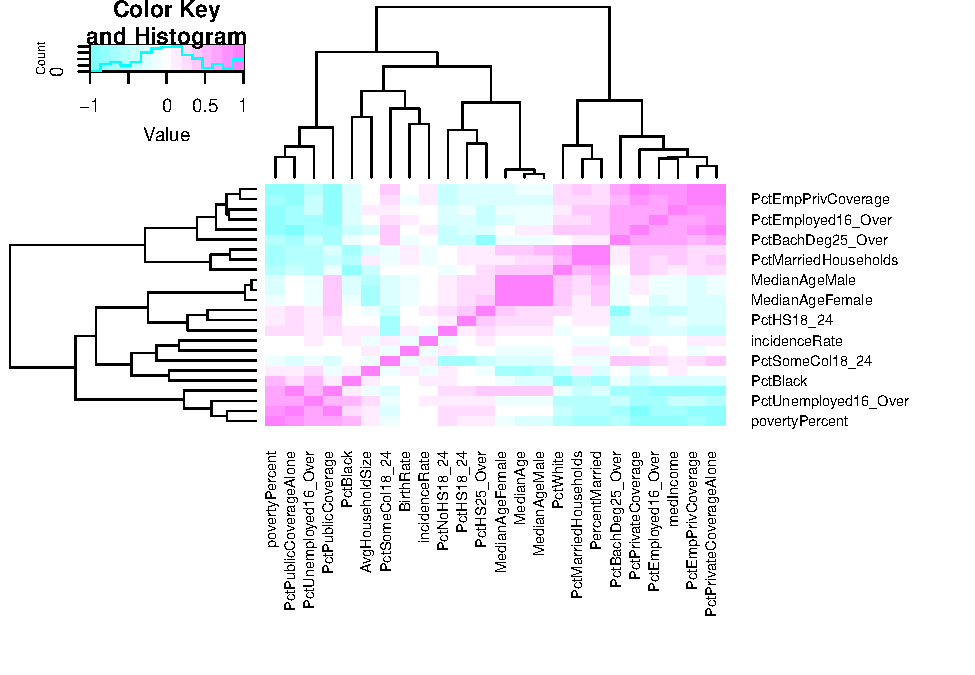
\includegraphics[width=0.7\linewidth]{report_files/figure-latex/unnamed-chunk-2-1} \end{center}

The \texttt{povertyPercent} variable correlates highly with other
predictors that deal with being under public insurance of being
unemployed. Conversely, poverty is highly negatively correlated with
having private insurance. The median ages of men and women are highly
correlated as well, so we will probably opt for just one of these. Since
the educational variable represent highest achievement, many of them are
correlated as well.

In making our future models, we now know that we'll have to deal with
this correlation and perform some model selection on our variables. We
performed an initial PCA to figure out what variables explained most of
the variance in average cancer mortality, and this will help guide our
final model selection.

\hypertarget{interaction-between-race-education}{%
\subsubsection{Interaction Between Race \&
Education}\label{interaction-between-race-education}}

One interesting trend that we found in the data was that there seemed to
be an interaction between race and education in relation to cancer
mortality. According to an article by the US Department of Education,
the median percentage of adults 25 and over completing a bachelor's
degree was 34\%. We divided the counties by if they fell below or were
equal to higher to the median value and investigated how cancer
mortality changed with percentage of race (Figure 2).

\begin{center}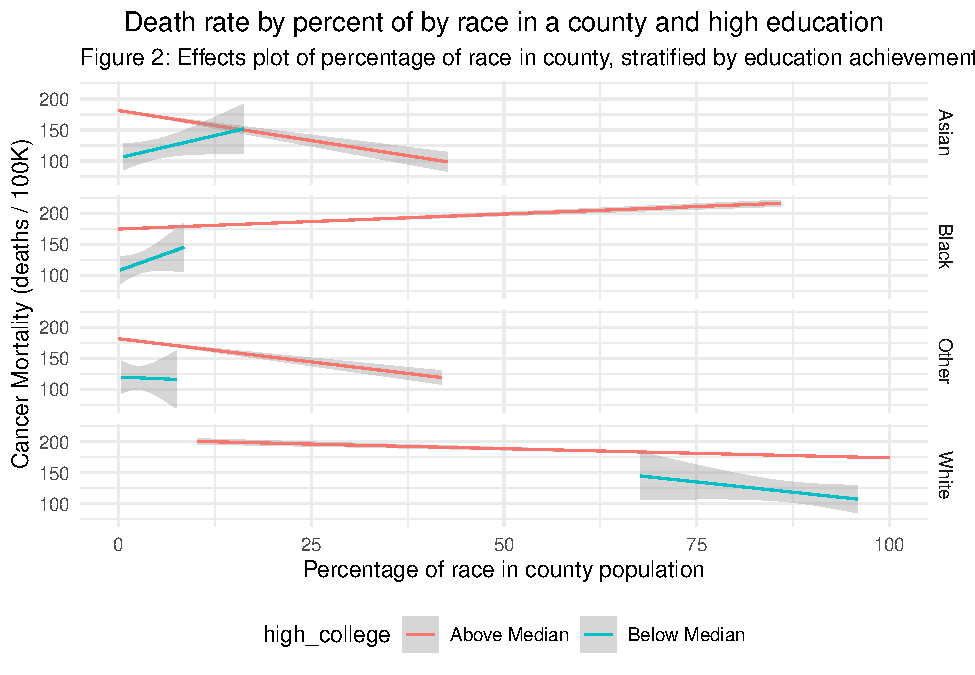
\includegraphics[width=0.7\linewidth]{report_files/figure-latex/unnamed-chunk-3-1} \end{center}

The change is most drastic in Asians, but the trend holds over all races
present in the data. For African-Americans, we also see an attenuation
of the average cancer mortality desite it not converting to a negative
correlation.

Based on the results of our exploratory analyses, we propose two
analytic questions:

\begin{enumerate}
\def\labelenumi{\arabic{enumi}.}
\tightlist
\item
  Can we identify county-level factors that contribute to a significant
  difference in cancer mortality? If so, can we identify any significant
  interaction between these factors that also contribute to increased
  cancer mortality?
\item
  Can we create an effective predictive model from the data? If we can
  find any significant interactions from our explanatory model, might
  they be helpful in increasing predictive ability?
\end{enumerate}

Our two questions is motivated by the nature of the data. The data is
contains most of the counties in the United States, so any estimates we
find apply directly to these counties during this time period. Since the
data is a ``snapshot'' of the population from 2011 - 2016, we must
acknowledge that the estimates we get in any explanatory model will
reflect population characteristics. We also acknowledge that some
variation is introduced because the data is come different points in
time, we assume that these measurements do not change drastically on the
scale of a few years. With the nature of the data in mind, we want to
try to use the explanatory model to see if any features or combination
of features might be useful in a prediction model, based on the
estimated coefficients.

\hypertarget{methodology}{%
\section{Methodology}\label{methodology}}

\hypertarget{explanatory-model}{%
\subsection{Explanatory Model}\label{explanatory-model}}

\hypertarget{model-selection}{%
\subsubsection{Model Selection}\label{model-selection}}

With 30 covariates, we tried a few different candidate models before
deciding on a final model. As seen in our correlation heatmap, we
decided on a subset of variables to use instead of creating combined
versions. Through a series of ANOVA, we found that an interaction model
contained significant interaction between education and race produced
the best fit in terms of adjusted \(R^2\), so this became a focal point
of our analysis.

Our final explanatory model is as follows:

\[
Y_i = X_{education}\beta + X_{race}\beta + X_{interaction}\beta + X_{confounders}\beta + \epsilon_i
\]

In terms of education variables, we chose 2 from the entire group: 1)
``percent of the county ages 25 and over finishing high school'', and 2)
the percent over 25 finishing college (bachelor's degree). For our race
variables, we included all that were present in the data (\% of the
county being Asian, Black, White or Other Race). With our literature
review and prior knowledge, we knew that age, sex, cancer incidence,
income, and population need to be accounted for in the model since they
are known confounders between cancer mortality and our covariates of
interest.

\hypertarget{analysis-plan}{%
\subsubsection{Analysis Plan}\label{analysis-plan}}

As mentioned before, the data concerning education and race come from
the 2013 Census. We know the the census data comes from a carefully
picked representative population in each county, but this information is
not available in the data itself. Despite the data containig most of the
counties in the United States, the randomness introduced by the survey
requires us to perform some inference. We expect there to be violations
to typical regression assumptions since adjacent counties may be
correlated. To account for this, we plan to use 1000 bootstrap samples
to calculate a robust confidence interval for each of the coefficients.
Coefficients that we find to be significant in the explanatory model
will be included in a prediction model candidate.

\hypertarget{prediction-model}{%
\subsection{Prediction Model}\label{prediction-model}}

We proceeded to build three models to predict county cancer death rates
using both the raw explanatory variables and interaction variables we
found to be significant. We built a lasso regularization, principal
component analysis (PCA), and forward backwards stepwise selection
model. We randomly split the data into 80\% train and 20\% test, and
then used this same split for all three models. Afterwards, for the
lasso and PCA models, the training set was further split into \(10\)
folds for cross-validation in order to tune the lambda and \(\#\) of PC
hyperparameters respectively. Choosing \(10\) folds and an \(80-20\)
split are usually default parameters in machine learning models.

\hypertarget{lasso}{%
\subsubsection{Lasso}\label{lasso}}

In lasso regularization, the aim is to minimize not just the residual
sum of squares (RSS), but the sum of RSS and a scalar multiple of the
absolute sum of the beta coefficients. This allows for the moderation of
beta coefficients and serves to filter out features that do minimal
explanation. We performed \(10\) fold cross-validation to select for the
optimal value of \(\lambda\), the scalar multiple, and then fitted the
lasso regularization model on the entire training set. The beta
estimates were then used to predict cancer death rates in the test set.

\hypertarget{pca}{%
\subsubsection{PCA}\label{pca}}

In PCA, we used \(10\) fold cross validation to select for an optimal
number of principal components (PCs). Since the error formula we used
was root mean square error (RMSE), adding additional PCs generally
decrease RMSE. As a result, we used a heuristic, the elbow rule, to
select for the optimal amount of PCs. The elbow rule selects an optimal
value for the number of PCs when adding additional PCs no longer
significantly reduces RMSE. Once we selected the optimal number of PCs,
\(k\), we computed the first \(k\) PC loadings and used those loadings
to predict the cancer death rates in the train and test sets.

\hypertarget{forward-and-backward-stepwise-selection}{%
\subsubsection{Forward and Backward Stepwise
Selection}\label{forward-and-backward-stepwise-selection}}

Forward and backwards stepwise selection did not use cross-validation to
select for a hyperparmeter. Instead, we used the stepwise selection
algorithm with AIC as a metric on the entire training set to select for
a set of variables. These variables were then fitted on the training set
and used to predict the cancer death rates in the test set.

\hypertarget{model-metrics}{%
\subsubsection{Model Metrics}\label{model-metrics}}

To assess each of these models, we computed the RMSE and \(R^2\) values
of the true cancer death rates versus predicted cancer death rates of
the training set. The model with the highest RMSE and/or \(R^2\) values
would then be the ideal model candidate to perform the test set
predictions. The estimated beta coefficients in the lasso and stepwise
models and the loadings in the PCA model can be used to interpret
prediction results.

\hypertarget{results-discussion}{%
\section{Results \& Discussion}\label{results-discussion}}

\hypertarget{initial-explanatory-model}{%
\subsubsection{Initial Explanatory
Model}\label{initial-explanatory-model}}

Table 2 shows the intial estimates for our final explanatory model.
Looking at the main effects, we see that with the exception of Asians,
higher proportions of the other races was associated with higher average
cancer mortality in a county. Most of the interaction terms are small
and insignificant, but most are associated with average decreases in
mortality. This lines up with previous research suggesting that
education is beneficial for health outcomes.

\begin{longtable}[]{@{}lrl@{}}
\caption{Estimated coefficients and 95\% CI}\tabularnewline
\toprule
term & estimate & 95\% CI\tabularnewline
\midrule
\endfirsthead
\toprule
term & estimate & 95\% CI\tabularnewline
\midrule
\endhead
pct\_hs25\_over & 2.870 & (2.26, 3.48)\tabularnewline
pct\_bach\_deg25\_over & 2.066 & (0.953, 3.179)\tabularnewline
pct\_white & 1.164 & (0.852, 1.476)\tabularnewline
pct\_black & 1.061 & (0.71, 1.412)\tabularnewline
pct\_asian & -0.589 & (-1.927, 0.749)\tabularnewline
pct\_other\_race & -1.507 & (-2.196, -0.819)\tabularnewline
pct\_hs25\_over:pct\_white & -0.026 & (-0.032, -0.019)\tabularnewline
pct\_hs25\_over:pct\_black & -0.032 & (-0.039, -0.025)\tabularnewline
pct\_hs25\_over:pct\_asian & 0.017 & (-0.011, 0.045)\tabularnewline
pct\_hs25\_over:pct\_other\_race & 0.014 & (-0.002, 0.03)\tabularnewline
pct\_bach\_deg25\_over:pct\_white & -0.041 & (-0.052,
-0.029)\tabularnewline
pct\_bach\_deg25\_over:pct\_black & -0.002 & (-0.014,
0.01)\tabularnewline
pct\_bach\_deg25\_over:pct\_asian & -0.006 & (-0.039,
0.027)\tabularnewline
pct\_bach\_deg25\_over:pct\_other\_race & 0.029 & (0.007,
0.052)\tabularnewline
\bottomrule
\end{longtable}

\hypertarget{interaction-between-education-race}{%
\subsubsection{Interaction Between Education \&
Race}\label{interaction-between-education-race}}

Figure 3 shows the 95\% bootstrap percentile intervals of 1000 bootstrap
interaction models. The bootstrap 95\% confidence intervals indicate
that only the high school interactions with African- and white Americans
were significant. The coefficients associated with these interactions
are all negative, hich matches with our original estimated model.

\begin{center}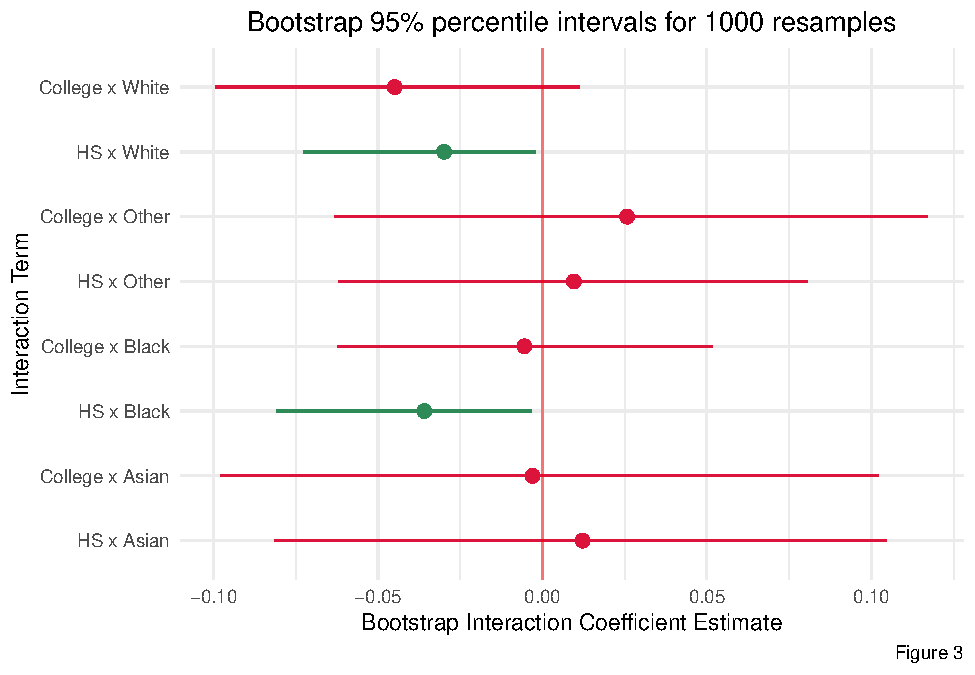
\includegraphics[width=0.7\linewidth]{report_files/figure-latex/bootstrap_table-1} \end{center}

With these findings, we include these two interaction terms inside of a
candidate predictive model.

\hypertarget{prediction-model-1}{%
\subsection{Prediction Model}\label{prediction-model-1}}

The lasso regularization model selected an optimal hyperparameter of
\(\lambda = 0.00119\) as shown in Figure X (a). The estimated
coefficients fitted from the training set are shown in Table Y, with
only the intercept and incidenceRate having coefficients of \(0\). The
training set RMSE and \(R^2\) was \(13.796\) and \(0.866\) respectively,
and the test set metrics showed slight improvements with an RMSE and
\(R^2\) of \(12.842\) and \(0.872\) respectively. These values are in
Table Z.

Using the elbow rule as shown in Figure C (a), we selected \(10\) PCs to
be the optimal amount and obtained the loadings of the first \(10\) PCs
from the training set. A summary of these loadings are in Table A, where
roughly half of the variables did not show up significantly in any of
the \(10\) PCs. The training set RMSE and \(R^2\) was \(20.020\) and
\(0.689\) respectively, and the test set metrics showed moderate
improvements with an RMSE and \(R^2\) of \(17.955\) and \(0.728\)
respectively.

Our stepwise selection model included \(23\) variables, and the order in
which they were selected is displayed in Figure B. The estimated
coefficients fitted from the training set are shown in Table Y along
with the lasso regularization coefficients. The training set RMSE and
\(R^2\) was \(13.278\) and \(0.877\) respectively, and the test set
metrics showed slight improvements with an RMSE and \(R^2\) of
\(12.495\) and \(0.879\) respectively. These values are in Table Z.

\begin{Shaded}
\begin{Highlighting}[]
\NormalTok{final_metrics}
\end{Highlighting}
\end{Shaded}

\begin{verbatim}
##                      Lasso        PCA   Stepwise
## R_squared_train  0.8664342  0.6892268  0.8769632
## R_squared_test   0.8718580  0.7281111  0.8794552
## RMSE_train      13.7961626 20.0200150 13.2783463
## RMSE_test       12.8424256 17.9551337 12.4945712
\end{verbatim}

Table Z

\begin{Shaded}
\begin{Highlighting}[]
\NormalTok{final_coeffs}
\end{Highlighting}
\end{Shaded}

\begin{verbatim}
##                                   step_coeffs  lasso_coeffs
## (Intercept)                      8.982813e+02            NA
## avgAnnCount_log                 -2.755781e+00 -1.914430e+00
## avgDeathsPerYear_log             1.039750e+02  1.121735e+02
## AvgHouseholdSize                 4.653770e+00  6.639897e+00
## BirthRate                       -4.772253e-01 -6.828285e-01
## college_black                    1.823608e-02  1.490543e-02
## hs_black                                   NA -2.201629e-02
## hs_white                                   NA -1.898820e-02
## Imputed_PctEmployed16_Over      -4.832461e-01 -6.286077e-01
## Imputed_PctPrivateCoverageAlone            NA -2.531996e-02
## incidenceRate                    9.508184e-02            NA
## MedianAge                       -2.559524e+00 -2.872336e+00
## medIncome                        3.834720e-04  5.224504e-04
## PctAsian_log                               NA  3.642454e-01
## PctBachDeg18_24_log                        NA  1.415853e-02
## PctBachDeg25_Over               -1.529700e-01 -1.637155e-01
## PctBlack                        -1.887251e-01  6.371510e-01
## PctEmployed16_Over              -5.092996e-01 -6.566720e-01
## PctEmpPrivCoverage               1.053615e-01  1.436310e-01
## PctHS18_24                       3.614372e-01  4.166293e-01
## PctHS25_Over                               NA  1.865748e+00
## PctMarriedHouseholds                       NA -4.685820e-01
## PctNoHS18_24                    -6.260260e-02 -4.481827e-02
## PctOtherRace_log                -9.016052e-01 -1.265590e+00
## PctPrivateCoverage              -2.662975e-01 -5.540287e-02
## PctPrivateCoverageAlone                    NA -2.523838e-02
## PctPublicCoverage               -2.148296e+00 -2.366866e+00
## PctPublicCoverageAlone           1.644217e+00  2.046082e+00
## PctSomeCol18_24                            NA  4.212474e-02
## PctUnemployed16_Over             8.859463e-01  9.699252e-01
## PctWhite                                   NA  6.649455e-01
## PercentMarried                             NA  4.895686e-01
## popEst2015_log                  -1.010836e+02 -1.093631e+02
## povertyPercent                   3.958523e-01  5.106701e-01
## studyPerCap_log                 -4.043149e-01 -3.224617e-01
\end{verbatim}

Table Y

\begin{Shaded}
\begin{Highlighting}[]
\KeywordTok{grid.arrange}\NormalTok{(g_lasso_hyper,g_lasso_train,g_lasso_test, }\DataTypeTok{layout_matrix =}\NormalTok{ lay1)}
\end{Highlighting}
\end{Shaded}

\begin{center}\includegraphics[width=0.7\linewidth]{report_files/figure-latex/unnamed-chunk-8-1} \end{center}

Figure X

\begin{Shaded}
\begin{Highlighting}[]
\KeywordTok{grid.arrange}\NormalTok{(g_pca_hyper,g_pca_train,g_pca_test, }\DataTypeTok{layout_matrix =}\NormalTok{ lay1)}
\end{Highlighting}
\end{Shaded}

\begin{center}\includegraphics[width=0.7\linewidth]{report_files/figure-latex/unnamed-chunk-9-1} \end{center}

Figure C

\begin{Shaded}
\begin{Highlighting}[]
\KeywordTok{grid.arrange}\NormalTok{(g_step_hyper,g_step_train,g_step_test, }\DataTypeTok{layout_matrix =}\NormalTok{ lay1)}
\end{Highlighting}
\end{Shaded}

\begin{center}\includegraphics[width=0.7\linewidth]{report_files/figure-latex/unnamed-chunk-10-1} \end{center}

Figure B

\begin{Shaded}
\begin{Highlighting}[]
\NormalTok{final_loadings}
\end{Highlighting}
\end{Shaded}

\begin{verbatim}
##                                           PC1           PC2           PC3
## incidenceRate                   -4.906072e-05 -3.458332e-03 -3.015126e-02
## medIncome                       -9.997924e-01 -9.091488e-03 -1.808253e-02
## povertyPercent                   4.154681e-04  2.494200e-03 -6.532604e-04
## MedianAge                        5.354222e-05 -2.276568e-03 -1.633544e-03
## AvgHouseholdSize                -3.305854e-06  7.998591e-05  7.136982e-05
## PercentMarried                  -1.940984e-04 -4.366232e-03  2.376839e-03
## PctNoHS18_24                     1.943937e-04  3.499056e-04 -1.201002e-03
## PctHS18_24                       1.413698e-04 -2.459173e-03 -4.519889e-03
## PctSomeCol18_24                 -1.525707e-04  1.671578e-03  5.033931e-03
## PctHS25_Over                     2.795490e-04 -4.569666e-03 -9.369580e-03
## PctBachDeg25_Over               -3.140969e-04  1.558766e-03  3.850017e-03
## PctEmployed16_Over              -4.460714e-04 -8.560957e-04  2.613779e-03
## PctUnemployed16_Over             1.257925e-04  1.369913e-03 -9.348405e-04
## PctPrivateCoverage              -6.329772e-04 -3.100880e-03 -1.845921e-03
## PctPrivateCoverageAlone         -5.243248e-04 -1.921167e-03 -2.888842e-03
## PctEmpPrivCoverage              -5.784454e-04 -1.658185e-03 -3.167077e-03
## PctPublicCoverage                4.895938e-04 -2.904349e-04 -8.102522e-04
## PctPublicCoverageAlone           3.625061e-04  1.211969e-03 -1.343620e-04
## PctWhite                        -2.063774e-04 -1.487998e-02  1.068190e-02
## PctBlack                         3.099063e-04  1.125577e-02 -2.284246e-02
## PctMarriedHouseholds            -2.352540e-04 -3.643326e-03  1.530868e-03
## BirthRate                        1.074871e-06 -4.212607e-05  4.317079e-04
## Imputed_PctEmployed16_Over      -2.847074e-05 -1.674489e-04  2.589367e-05
## Imputed_PctPrivateCoverageAlone -1.284187e-04  3.555906e-04  1.339068e-03
## avgAnnCount_log                 -4.106676e-05  2.866863e-04  1.968440e-04
## avgDeathsPerYear_log            -2.932705e-05  3.535126e-04 -5.207280e-06
## popEst2015_log                  -4.137450e-05  4.698798e-04  1.573582e-04
## studyPerCap_log                 -5.279787e-05  5.119546e-04  6.458466e-04
## PctBachDeg18_24_log             -3.946729e-05 -7.634365e-06 -2.046766e-06
## PctAsian_log                    -5.319556e-05  4.846992e-04  7.354057e-04
## PctOtherRace_log                -2.661135e-05  6.287687e-04  1.066399e-03
## hs_black                         1.324916e-02  3.712419e-01 -8.961406e-01
## hs_white                         1.538265e-02 -9.184454e-01 -3.920328e-01
## college_black                    8.043098e-04  1.345255e-01 -2.029164e-01
##                                           PC4           PC5           PC6
## incidenceRate                   -0.1255511821 -0.9900370682 -2.777466e-03
## medIncome                        0.0018017033  0.0004180523  3.653353e-04
## povertyPercent                   0.0028421778 -0.0022597616  2.017156e-03
## MedianAge                        0.0039004749  0.0035773653  6.917757e-03
## AvgHouseholdSize                 0.0002758510  0.0005120483 -6.476944e-05
## PercentMarried                   0.0076749257  0.0123081795  2.583746e-03
## PctNoHS18_24                     0.0187182942  0.0238726600  1.143759e-02
## PctHS18_24                       0.0124774176  0.0022677496  8.203723e-03
## PctSomeCol18_24                 -0.0215893978 -0.0236167538 -1.974094e-02
## PctHS25_Over                     0.0069497850 -0.0004548677 -1.854448e-03
## PctBachDeg25_Over               -0.0112663844  0.0003074223 -4.326691e-04
## PctEmployed16_Over              -0.0096115494 -0.0020518776 -5.214565e-02
## PctUnemployed16_Over            -0.0009041992 -0.0062921095  3.561810e-03
## PctPrivateCoverage              -0.0133579997 -0.0123139952 -1.821871e-02
## PctPrivateCoverageAlone         -0.0258428205 -0.0002829178 -7.158744e-01
## PctEmpPrivCoverage              -0.0115737697 -0.0194228541 -2.090703e-02
## PctPublicCoverage                0.0061966160 -0.0096855947  1.467622e-02
## PctPublicCoverageAlone           0.0038969118 -0.0085416665  8.455444e-03
## PctWhite                         0.0045601310 -0.0008443664  3.706167e-03
## PctBlack                        -0.0181169256  0.0019457048 -3.278570e-04
## PctMarriedHouseholds             0.0115806759  0.0183592422  3.111408e-03
## BirthRate                        0.0016154594  0.0034117913 -1.556177e-03
## Imputed_PctEmployed16_Over       0.0004241153  0.0004273098  3.811283e-02
## Imputed_PctPrivateCoverageAlone  0.0127661961 -0.0118908930  6.933157e-01
## avgAnnCount_log                 -0.0043110555 -0.0076358730 -3.195946e-04
## avgDeathsPerYear_log            -0.0047189107 -0.0055666361  5.632209e-04
## popEst2015_log                  -0.0046594854 -0.0044140687  1.964825e-04
## studyPerCap_log                 -0.0061135801 -0.0081772362 -1.601379e-03
## PctBachDeg18_24_log             -0.0025683251 -0.0027085191 -2.762398e-04
## PctAsian_log                    -0.0031996503 -0.0037813205  5.982809e-04
## PctOtherRace_log                 0.0004946635  0.0029924298  1.575223e-04
## hs_black                         0.2407662093 -0.0049660609 -5.150274e-03
## hs_white                        -0.0431873798  0.0205089081  4.010692e-03
## college_black                   -0.9598320345  0.1289877930  2.944341e-02
##                                           PC7           PC8          PC9
## incidenceRate                    8.684042e-03 -0.0362244361  0.010503239
## medIncome                        4.215921e-04 -0.0006410941 -0.001062094
## povertyPercent                   2.347184e-02 -0.0493721909 -0.175035031
## MedianAge                        1.086476e-02 -0.0579780527  0.040064365
## AvgHouseholdSize                 1.281368e-03 -0.0042882614 -0.005825779
## PercentMarried                  -1.232634e-02 -0.0352419083  0.222312821
## PctNoHS18_24                     5.348475e-02 -0.2978725600 -0.018240160
## PctHS18_24                       5.235641e-02 -0.4090464090  0.378464123
## PctSomeCol18_24                 -8.405795e-02  0.6470790612 -0.385483708
## PctHS25_Over                     7.995668e-03 -0.0670639649 -0.068593215
## PctBachDeg25_Over               -1.542547e-02  0.0898985113  0.098110418
## PctEmployed16_Over              -7.384286e-01 -0.0487841914  0.080810802
## PctUnemployed16_Over             2.556550e-02 -0.0486391980 -0.136751994
## PctPrivateCoverage              -7.135685e-02  0.2971863081  0.430311919
## PctPrivateCoverageAlone          1.337967e-02  0.1210674635  0.171786181
## PctEmpPrivCoverage              -5.939348e-02  0.2274566552  0.220673500
## PctPublicCoverage                5.032986e-02 -0.1523415894 -0.296553295
## PctPublicCoverageAlone           3.935570e-02 -0.1377931042 -0.301524414
## PctWhite                        -2.445263e-02  0.1853862365  0.233797227
## PctBlack                         2.596978e-04 -0.0022852438 -0.009117773
## PctMarriedHouseholds             8.846414e-03 -0.0382077150  0.155803426
## BirthRate                       -5.992504e-04 -0.0123443431  0.012765385
## Imputed_PctEmployed16_Over       6.471937e-01  0.1949936729  0.168645045
## Imputed_PctPrivateCoverageAlone -8.700357e-02  0.1597378723  0.184952549
## avgAnnCount_log                 -2.049905e-03  0.0137421327 -0.013572889
## avgDeathsPerYear_log             1.312474e-03  0.0070592335 -0.028896743
## popEst2015_log                   1.136788e-03  0.0090853176 -0.028487186
## studyPerCap_log                 -5.118682e-03  0.0312387434 -0.006062260
## PctBachDeg18_24_log             -7.436677e-03  0.0215244811  0.009266532
## PctAsian_log                    -6.034725e-05  0.0140037090 -0.014666663
## PctOtherRace_log                 1.213401e-04 -0.0109537158 -0.011731918
## hs_black                        -5.850860e-03  0.0154101544  0.002850570
## hs_white                         5.850028e-05  0.0004046477 -0.008784993
## college_black                    9.630910e-03 -0.0282457621  0.001764177
##                                          PC10
## incidenceRate                   -2.860960e-02
## medIncome                        2.450144e-05
## povertyPercent                   7.610751e-02
## MedianAge                       -2.193138e-01
## AvgHouseholdSize                 6.782392e-03
## PercentMarried                  -2.738575e-01
## PctNoHS18_24                    -5.794527e-01
## PctHS18_24                       5.212191e-01
## PctSomeCol18_24                  7.143079e-02
## PctHS25_Over                     1.300351e-01
## PctBachDeg25_Over               -4.895124e-02
## PctEmployed16_Over               6.896812e-03
## PctUnemployed16_Over             6.033483e-02
## PctPrivateCoverage              -5.500194e-02
## PctPrivateCoverageAlone          3.492956e-02
## PctEmpPrivCoverage               1.929601e-01
## PctPublicCoverage               -8.237150e-02
## PctPublicCoverageAlone           6.340484e-02
## PctWhite                        -3.661139e-01
## PctBlack                        -8.113672e-03
## PctMarriedHouseholds            -1.967987e-01
## BirthRate                       -4.485164e-03
## Imputed_PctEmployed16_Over       2.365081e-02
## Imputed_PctPrivateCoverageAlone  5.224743e-02
## avgAnnCount_log                  1.821538e-02
## avgDeathsPerYear_log             3.292264e-02
## popEst2015_log                   3.977256e-02
## studyPerCap_log                  3.521042e-02
## PctBachDeg18_24_log              1.576685e-02
## PctAsian_log                     3.704192e-02
## PctOtherRace_log                 1.549598e-02
## hs_black                        -5.747527e-03
## hs_white                         2.499088e-03
## college_black                   -1.226432e-02
\end{verbatim}

Table A

\hypertarget{conclusion}{%
\section{Conclusion}\label{conclusion}}

Our analysis found at least one significant interaction between race and
education that served to help reduce cancer mortality per capita on a
county level. Although this effect was small, their significance was
supported simultaneously by the model itself, the Wald test, and the
95\% bootstrap percentile intervals. These results support the
hypothesis that higher education has a beneficial effect on cancer
mortatlity, at least on the county scale. Furthermore, our findings are
in line with a wealth of literature that suggest that education is
beneficial to improving health outcomes.

The stepwise selection model showed the best RMSE and \(R^2\) in the
training set. Therefore, we select the stepwise selection model to
predict cancer death rates for the test set. We also see that the
stepwise selection model had the best metrics for the test set. The
stepwise selection model also included less beta coefficients (\(24\))
than the lasso regularization model (\(33\)), so it's much more
parsimonious than lasso which had marginally worse prediction metrics.
Most variables in the stepwise selection model had statistically
significant betas which are indicators of cancer death rates.

These findings are limited by the fact that the observational unit of
the data was a county. The model suggests a beneficial benefit, but does
not elucidate any reason as to why or how education interacts with race
to reduce cancer mortality among African- and white Americans. The
educational and race data come from 2013, so the model may be limited in
its generalizability to future years, especially in the context of
changing demographics and new educational environments created by
COVID-19. In light of these weaknesses, we feel that our model offers an
interesting perspective on how different demographic factors interact to
affect a health-related outcome. Being so prevalent, it's important to
understand these factors and interactions so that we can design proper
interventions.

\pagebreak

\hypertarget{references}{%
\section{References}\label{references}}

\begin{enumerate}
\def\labelenumi{\arabic{enumi}.}
\item
\item
\item
  ADLER, N.E. and OSTROVE, J.M. (1999), Socioeconomic Status and Health:
  What We Know and What We Don't. Annals of the New York Academy of
  Sciences, 896: 3-15.
  \url{https://doi.org/10.1111/j.1749-6632.1999.tb08101.x}
\item
  Rawl SM, Dickinson S, Lee JL, Roberts JL, Teal E, Baker LB, Kianersi
  S, Haggstrom DA. Racial and Socioeconomic Disparities in
  Cancer-Related Knowledge, Beliefs, and Behaviors in Indiana. Cancer
  Epidemiol Biomarkers Prev. 2019 Mar;28(3):462-470. doi:
  10.1158/1055-9965.EPI-18-0795. Epub 2018 Nov 28. PMID: 30487135.
\item
  Rohlfing ML, Mays AC, Isom S, Waltonen JD. Insurance status as a
  predictor of mortality in patients undergoing head and neck cancer
  surgery. Laryngoscope. 2017 Dec;127(12):2784-2789. doi:
  10.1002/lary.26713. Epub 2017 Jun 22. PMID: 28639701; PMCID:
  PMC5688011.
\item
  Zeigler-Johnson C, Keith S, McIntire R, Robinson T, Leader A, Glanz K.
  Racial and Ethnic Trends in Prostate Cancer Incidence and Mortality in
  Philadelphia, PA: an Observational Study. J Racial Ethn Health
  Disparities. 2019 Apr;6(2):371-379. doi: 10.1007/s40615-018-00534-z.
  Epub 2018 Dec 5. PMID: 30520002.
\item
  Singh, Gopal \& Jemal, Ahmedin. (2017). Socioeconomic and
  Racial/Ethnic Disparities in Cancer Mortality, Incidence, and Survival
  in the United States, 1950--2014: Over Six Decades of Changing
  Patterns and Widening Inequalities. Journal of Environmental and
  Public Health. 2017. 1-19. 10.1155/2017/2819372.
\item
  Mokdad AH, Dwyer-Lindgren L, Fitzmaurice C, et al.~Trends and Patterns
  of Disparities in Cancer Mortality Among US Counties, 1980-2014. JAMA.
  2017;317(4):388--406. \url{doi:10.1001/jama.2016.20324}
\item
  \url{https://nces.ed.gov/pubs93/93442.pdf}
\end{enumerate}

\pagebreak

\hypertarget{appendix}{%
\section{Appendix}\label{appendix}}

\begin{Shaded}
\begin{Highlighting}[]
\KeywordTok{library}\NormalTok{(tidyverse)}
\KeywordTok{library}\NormalTok{(knitr)}
\KeywordTok{library}\NormalTok{(gplots)}
\KeywordTok{library}\NormalTok{(gridExtra)}
\KeywordTok{library}\NormalTok{(glmnet)}
\KeywordTok{library}\NormalTok{(grid)}
\KeywordTok{library}\NormalTok{(caret)}
\KeywordTok{library}\NormalTok{(olsrr)}

\KeywordTok{set.seed}\NormalTok{(}\DecValTok{1}\NormalTok{)}

\NormalTok{knitr}\OperatorTok{::}\NormalTok{opts_chunk}\OperatorTok{$}\KeywordTok{set}\NormalTok{(}
  \DataTypeTok{fig.align =} \StringTok{"center"}\NormalTok{,}
  \DataTypeTok{out.width =} \StringTok{"70%"}
\NormalTok{)}

\CommentTok{# Load the data and do some processing}
\NormalTok{cancer =}\StringTok{ }\KeywordTok{read_csv}\NormalTok{(}\StringTok{"cancer_registry.csv"}\NormalTok{) }\OperatorTok\StringTok{ }
\StringTok{  }\CommentTok{# Split the geography variable}
\StringTok{  }\KeywordTok{separate}\NormalTok{(Geography, }\DataTypeTok{into =} \KeywordTok{c}\NormalTok{(}\StringTok{"county"}\NormalTok{, }\StringTok{"state"}\NormalTok{), }\DataTypeTok{sep =} \StringTok{", "}\NormalTok{) }\OperatorTok\StringTok{ }
\StringTok{  }\CommentTok{# Split up binnedInc into a lower and upper decile}
\StringTok{  }\KeywordTok{mutate}\NormalTok{(}
    \DataTypeTok{binnedInc =} \KeywordTok{str_remove_all}\NormalTok{(binnedInc, }\StringTok{"[(}\CharTok{\textbackslash{}\textbackslash{}}\StringTok{]]"}\NormalTok{),}
    \CommentTok{# also try to group states by region}
    \DataTypeTok{region =} \KeywordTok{case_when}\NormalTok{(}
\NormalTok{      state }\OperatorTok\StringTok{ }\KeywordTok{c}\NormalTok{(}\StringTok{"California"}\NormalTok{, }\StringTok{"Oregon"}\NormalTok{, }\StringTok{"Washington"}\NormalTok{, }\StringTok{"Nevada"}\NormalTok{, }\StringTok{"Idaho"}\NormalTok{, }
                   \StringTok{"Montana"}\NormalTok{, }\StringTok{"Wyoming"}\NormalTok{, }\StringTok{"Colorado"}\NormalTok{, }\StringTok{"Utah"}\NormalTok{, }\StringTok{"Alaska"}\NormalTok{, }\StringTok{"Hawaii"}\NormalTok{) }\OperatorTok{~}\StringTok{ "West"}\NormalTok{,}
\NormalTok{      state }\OperatorTok\StringTok{ }\KeywordTok{c}\NormalTok{(}\StringTok{"Arizona"}\NormalTok{, }\StringTok{"New Mexico"}\NormalTok{, }\StringTok{"Texas"}\NormalTok{, }\StringTok{"Oklahoma"}\NormalTok{) }\OperatorTok{~}\StringTok{ "Southwest"}\NormalTok{,}
\NormalTok{      state }\OperatorTok\StringTok{ }\KeywordTok{c}\NormalTok{(}\StringTok{"North Dakota"}\NormalTok{, }\StringTok{"South Dakota"}\NormalTok{, }\StringTok{"Nebraska"}\NormalTok{, }\StringTok{"Kansas"}\NormalTok{, }
                   \StringTok{"Minnesota"}\NormalTok{, }\StringTok{"Iowa"}\NormalTok{, }\StringTok{"Missouri"}\NormalTok{, }\StringTok{"Wisconsin"}\NormalTok{, }\StringTok{"Illinois"}\NormalTok{, }
                   \StringTok{"Indiana"}\NormalTok{, }\StringTok{"Ohio"}\NormalTok{, }\StringTok{"Michigan"}\NormalTok{) }\OperatorTok{~}\StringTok{ "Midwest"}\NormalTok{,}
\NormalTok{      state }\OperatorTok\StringTok{ }\KeywordTok{c}\NormalTok{(}\StringTok{"Arkansas"}\NormalTok{, }\StringTok{"Louisiana"}\NormalTok{, }\StringTok{"Mississippi"}\NormalTok{, }\StringTok{"Alabama"}\NormalTok{, }\StringTok{"Georgia"}\NormalTok{,}
                   \StringTok{"Florida"}\NormalTok{, }\StringTok{"South Carolina"}\NormalTok{, }\StringTok{"North Carolina"}\NormalTok{, }\StringTok{"Tennessee"}\NormalTok{,}
                   \StringTok{"Kentucky"}\NormalTok{, }\StringTok{"Virginia"}\NormalTok{, }\StringTok{"West Virginia"}\NormalTok{, }\StringTok{"District of Columbia"}\NormalTok{,}
                   \StringTok{"Delaware"}\NormalTok{) }\OperatorTok{~}\StringTok{ "Southeast"}\NormalTok{,}
\NormalTok{      state }\OperatorTok\StringTok{ }\KeywordTok{c}\NormalTok{(}\StringTok{"Maryland"}\NormalTok{, }\StringTok{"Pennsylvania"}\NormalTok{, }\StringTok{"New Jersey"}\NormalTok{, }\StringTok{"New York"}\NormalTok{, }\StringTok{"Rhode Island"}\NormalTok{,}
                   \StringTok{"Connecticut"}\NormalTok{, }\StringTok{"Massachusetts"}\NormalTok{, }\StringTok{"New Hampshire"}\NormalTok{, }\StringTok{"Vermont"}\NormalTok{, }\StringTok{"Maine"}\NormalTok{) }\OperatorTok{~}\StringTok{ "Northeast"}\NormalTok{,}
      \OtherTok{TRUE} \OperatorTok{~}\StringTok{ "Southwest"} \CommentTok{# Weird formatting means a single NM is NA in state}
\NormalTok{    )}
\NormalTok{  ) }\OperatorTok\StringTok{ }
\StringTok{  }\KeywordTok{separate}\NormalTok{(binnedInc, }\DataTypeTok{into =} \KeywordTok{c}\NormalTok{(}\StringTok{"inc_dec_low"}\NormalTok{, }\StringTok{"inc_dec_high"}\NormalTok{), }\DataTypeTok{sep =} \StringTok{","}\NormalTok{) }\OperatorTok\StringTok{ }
\StringTok{  }\NormalTok{janitor}\OperatorTok{::}\KeywordTok{clean_names}\NormalTok{() }\OperatorTok\StringTok{  }\CommentTok{# Convert all column names to lowercase'}
\StringTok{  }\KeywordTok{mutate}\NormalTok{(}
    \DataTypeTok{high_college =}\NormalTok{ pct_bach_deg25_over }\OperatorTok{>}\StringTok{ }\KeywordTok{median}\NormalTok{(pct_bach_deg25_over), }\CommentTok{# median(pct_bach_deg18_24),}
    \DataTypeTok{high_hs =}\NormalTok{ pct_hs18_}\DecValTok{24} \OperatorTok{>}\StringTok{ }\KeywordTok{median}\NormalTok{(pct_hs18_}\DecValTok{24}\NormalTok{)}
\NormalTok{  )}
\NormalTok{df <-}\StringTok{ }\KeywordTok{read.csv}\NormalTok{(}\StringTok{'cancer_registry.csv'}\NormalTok{) }\OperatorTok
\StringTok{  }\KeywordTok{mutate}\NormalTok{(}\DataTypeTok{PctSomeCol18_24 =} \DecValTok{100} \OperatorTok{-}\StringTok{ }\NormalTok{PctNoHS18_}\DecValTok{24} \OperatorTok{-}\StringTok{ }\NormalTok{PctHS18_}\DecValTok{24} \OperatorTok{-}\StringTok{ }\NormalTok{PctBachDeg18_}\DecValTok{24}\NormalTok{) }\OperatorTok
\StringTok{  }\KeywordTok{filter}\NormalTok{(incidenceRate }\OperatorTok{<}\StringTok{ }\DecValTok{1000}\NormalTok{) }\OperatorTok
\StringTok{  }\KeywordTok{filter}\NormalTok{(avgAnnCount }\OperatorTok{<}\StringTok{ }\DecValTok{20000}\NormalTok{) }\OperatorTok
\StringTok{  }\KeywordTok{filter}\NormalTok{(MedianAge }\OperatorTok{<}\StringTok{ }\DecValTok{200}\NormalTok{) }\OperatorTok
\StringTok{  }\KeywordTok{filter}\NormalTok{(AvgHouseholdSize }\OperatorTok{>}\StringTok{ }\DecValTok{1}\NormalTok{)}

\NormalTok{df <-}\StringTok{ }\KeywordTok{na.omit}\NormalTok{(df)}
\NormalTok{vars <-}\StringTok{ }\KeywordTok{colnames}\NormalTok{(df)}
\NormalTok{misc_vars <-}\StringTok{ }\KeywordTok{c}\NormalTok{(}\StringTok{'binnedInc'}\NormalTok{, }\StringTok{'Geography'}\NormalTok{, }\StringTok{'TARGET_deathRate'}\NormalTok{)}
\NormalTok{vars_}\DecValTok{1}\NormalTok{ <-}\StringTok{ }\KeywordTok{setdiff}\NormalTok{(vars, misc_vars)}
\NormalTok{log_vars <-}\StringTok{ }\KeywordTok{c}\NormalTok{(}\StringTok{'avgAnnCount'}\NormalTok{, }\StringTok{'avgDeathsPerYear'}\NormalTok{, }\StringTok{'popEst2015'}\NormalTok{, }\StringTok{'studyPerCap'}\NormalTok{, }\StringTok{'PctBachDeg18_24'}\NormalTok{, }\StringTok{'PctAsian'}\NormalTok{, }\StringTok{'PctOtherRace'}\NormalTok{)}
\NormalTok{log_names <-}\StringTok{ }\KeywordTok{c}\NormalTok{()}

\NormalTok{all_vars <-}\StringTok{ }\KeywordTok{setdiff}\NormalTok{(vars_}\DecValTok{1}\NormalTok{, log_vars)}
\NormalTok{all_vars <-}\StringTok{ }\KeywordTok{append}\NormalTok{(all_vars, log_names)}
\NormalTok{all_vars <-}\StringTok{ }\KeywordTok{sort}\NormalTok{(all_vars)}

\NormalTok{df_temp <-}\StringTok{ }\NormalTok{df }\OperatorTok\StringTok{ }\KeywordTok{select}\NormalTok{(all_vars)}
\NormalTok{df_temp <-}\StringTok{ }\KeywordTok{na.omit}\NormalTok{(df_temp)}

\NormalTok{heatmap2 <-}\StringTok{ }\KeywordTok{cor}\NormalTok{(df_temp)}
\KeywordTok{heatmap.2}\NormalTok{(heatmap2, }\DataTypeTok{trace =} \StringTok{'none'}\NormalTok{, }\DataTypeTok{margins =} \KeywordTok{c}\NormalTok{(}\DecValTok{10}\NormalTok{,}\DecValTok{10}\NormalTok{), }\DataTypeTok{col =} \StringTok{'cm.colors'}\NormalTok{, }\DataTypeTok{cexRow=}\FloatTok{0.7}\NormalTok{, }\DataTypeTok{cexCol =} \FloatTok{0.7}\NormalTok{)}
\NormalTok{cancer }\OperatorTok\StringTok{ }
\StringTok{  }\KeywordTok{mutate}\NormalTok{(}
    \DataTypeTok{high_college =}\NormalTok{ pct_bach_deg25_over }\OperatorTok{>}\StringTok{ }\DecValTok{34}\NormalTok{, }\CommentTok{# median(pct_bach_deg18_24),}
\NormalTok{  ) }\OperatorTok\StringTok{ }
\StringTok{  }\KeywordTok{pivot_longer}\NormalTok{(}
    \DataTypeTok{cols =} \KeywordTok{c}\NormalTok{(}\StringTok{"pct_white"}\NormalTok{, }
             \StringTok{"pct_black"}\NormalTok{, }
             \StringTok{"pct_asian"}\NormalTok{,}
             \StringTok{"pct_other_race"}\NormalTok{),}
    \DataTypeTok{values_to =} \StringTok{"pct"}\NormalTok{,}
    \DataTypeTok{names_to =} \StringTok{"race"}
\NormalTok{  ) }\OperatorTok\StringTok{ }
\StringTok{  }\KeywordTok{mutate}\NormalTok{(}
    \DataTypeTok{race =} \KeywordTok{case_when}\NormalTok{(}
\NormalTok{      race }\OperatorTok{==}\StringTok{ "pct_white"} \OperatorTok{~}\StringTok{ "White"}\NormalTok{,}
\NormalTok{      race }\OperatorTok{==}\StringTok{ "pct_black"} \OperatorTok{~}\StringTok{ "Black"}\NormalTok{,}
\NormalTok{      race }\OperatorTok{==}\StringTok{ "pct_asian"} \OperatorTok{~}\StringTok{ "Asian"}\NormalTok{,}
\NormalTok{      race }\OperatorTok{==}\StringTok{ "pct_other_race"} \OperatorTok{~}\StringTok{ "Other"}
\NormalTok{    )}
\NormalTok{  ) }\OperatorTok\StringTok{ }
\StringTok{  }\KeywordTok{ggplot}\NormalTok{(}\KeywordTok{aes}\NormalTok{(}\DataTypeTok{x =}\NormalTok{ pct, }\DataTypeTok{y =}\NormalTok{ target_death_rate, }\DataTypeTok{color =}\NormalTok{ high_college)) }\OperatorTok{+}\StringTok{ }
\StringTok{  }\KeywordTok{geom_smooth}\NormalTok{(}\DataTypeTok{method =} \StringTok{"lm"}\NormalTok{, }\DataTypeTok{size =} \FloatTok{0.5}\NormalTok{) }\OperatorTok{+}
\StringTok{  }\KeywordTok{facet_grid}\NormalTok{(race }\OperatorTok{~}\StringTok{ }\NormalTok{.) }\OperatorTok{+}
\StringTok{  }\KeywordTok{theme_minimal}\NormalTok{() }\OperatorTok{+}
\StringTok{  }\KeywordTok{theme}\NormalTok{(}
    \DataTypeTok{legend.position =} \StringTok{"bottom"}\NormalTok{,}
    \DataTypeTok{plot.title =} \KeywordTok{element_text}\NormalTok{(}\DataTypeTok{hjust =} \FloatTok{0.5}\NormalTok{)}
\NormalTok{  ) }\OperatorTok{+}\StringTok{ }
\StringTok{  }\KeywordTok{labs}\NormalTok{(}
    \DataTypeTok{title =} \StringTok{"Death rate by percent of by race in a county and high education"}\NormalTok{,}
    \DataTypeTok{subtitle =} \StringTok{"Figure 2: Effects plot of percentage of race in county, stratified by education achievement"}\NormalTok{,}
    \DataTypeTok{x =} \StringTok{"Percentage of race in county population"}\NormalTok{,}
    \DataTypeTok{y =} \StringTok{"Cancer Mortality (deaths / 100K)"}\NormalTok{) }\OperatorTok{+}
\StringTok{  }\KeywordTok{scale_color_discrete}\NormalTok{(}\DataTypeTok{labels =} \KeywordTok{c}\NormalTok{(}\StringTok{"Above Median"}\NormalTok{, }\StringTok{"Below Median"}\NormalTok{)) }
\NormalTok{cancer_model =}\StringTok{ }\KeywordTok{lm}\NormalTok{(target_death_rate }\OperatorTok{~}\StringTok{ }\NormalTok{pct_hs25_over }\OperatorTok{+}\StringTok{ }\NormalTok{pct_bach_deg25_over }\OperatorTok{+}\StringTok{ }
\StringTok{             }\NormalTok{pct_white }\OperatorTok{+}\StringTok{ }\NormalTok{pct_black }\OperatorTok{+}\StringTok{ }\NormalTok{pct_asian }\OperatorTok{+}\StringTok{ }\NormalTok{pct_other_race }\OperatorTok{+}
\StringTok{             }\CommentTok{# Interactions}
\StringTok{             }\NormalTok{pct_white}\OperatorTok{*}\NormalTok{pct_hs25_over }\OperatorTok{+}\StringTok{ }\NormalTok{pct_black}\OperatorTok{*}\NormalTok{pct_hs25_over }\OperatorTok{+}\StringTok{ }\NormalTok{pct_asian}\OperatorTok{*}\NormalTok{pct_hs25_over }\OperatorTok{+}\StringTok{ }\NormalTok{pct_other_race}\OperatorTok{*}\NormalTok{pct_hs25_over }\OperatorTok{+}
\StringTok{             }\NormalTok{pct_white}\OperatorTok{*}\NormalTok{pct_bach_deg25_over }\OperatorTok{+}\StringTok{ }\NormalTok{pct_black}\OperatorTok{*}\NormalTok{pct_bach_deg25_over }\OperatorTok{+}\StringTok{ }\NormalTok{pct_asian}\OperatorTok{*}\NormalTok{pct_bach_deg25_over }\OperatorTok{+}\StringTok{ }\NormalTok{pct_other_race}\OperatorTok{*}\NormalTok{pct_bach_deg25_over }\OperatorTok{+}
\StringTok{             }\CommentTok{# Confounders}
\StringTok{             }\NormalTok{incidence_rate }\OperatorTok{+}\StringTok{ }\NormalTok{med_income }\OperatorTok{+}\StringTok{ }\NormalTok{pop_est2015 }\OperatorTok{+}\StringTok{ }\NormalTok{poverty_percent }\OperatorTok{+}\StringTok{ }\NormalTok{median_age,}
           \DataTypeTok{data =}\NormalTok{ cancer)}

\NormalTok{cancer_model }\OperatorTok\StringTok{ }
\StringTok{  }\NormalTok{broom}\OperatorTok{::}\KeywordTok{tidy}\NormalTok{() }\OperatorTok\StringTok{ }
\StringTok{  }\KeywordTok{mutate}\NormalTok{(}
    \DataTypeTok{left =}\NormalTok{ estimate }\OperatorTok{-}\StringTok{ }\KeywordTok{qt}\NormalTok{(}\FloatTok{0.75}\NormalTok{, }\DataTypeTok{df =} \KeywordTok{nrow}\NormalTok{(cancer) }\OperatorTok{-}\StringTok{ }\KeywordTok{length}\NormalTok{(cancer_model}\OperatorTok{$}\NormalTok{coefficients)) }\OperatorTok{*}\StringTok{ }\NormalTok{std.error,}
    \DataTypeTok{right =}\NormalTok{ estimate }\OperatorTok{+}\StringTok{ }\KeywordTok{qt}\NormalTok{(}\FloatTok{0.75}\NormalTok{, }\DataTypeTok{df =} \KeywordTok{nrow}\NormalTok{(cancer) }\OperatorTok{-}\StringTok{ }\KeywordTok{length}\NormalTok{(cancer_model}\OperatorTok{$}\NormalTok{coefficients)) }\OperatorTok{*}\StringTok{ }\NormalTok{std.error,}
    \StringTok{`}\DataTypeTok{95% CI}\StringTok{`}\NormalTok{ =}\StringTok{ }\KeywordTok{paste0}\NormalTok{(}\StringTok{"("}\NormalTok{, left }\OperatorTok\StringTok{ }\KeywordTok{round}\NormalTok{(}\DecValTok{3}\NormalTok{), }\StringTok{", "}\NormalTok{, right }\OperatorTok\StringTok{ }\KeywordTok{round}\NormalTok{(}\DecValTok{3}\NormalTok{), }\StringTok{")"}\NormalTok{)}
\NormalTok{  ) }\OperatorTok\StringTok{ }
\StringTok{  }\KeywordTok{filter}\NormalTok{(}
\NormalTok{    term }\OperatorTok\StringTok{ }\KeywordTok{c}\NormalTok{(}\StringTok{"pct_hs25_over"}\NormalTok{, }\StringTok{"pct_bach_deg25_over"}\NormalTok{,}
                \StringTok{"pct_white"}\NormalTok{, }\StringTok{"pct_black"}\NormalTok{, }\StringTok{"pct_asian"}\NormalTok{, }\StringTok{"pct_other_race"}\NormalTok{,}
                \StringTok{"pct_hs25_over:pct_white"}\NormalTok{, }\StringTok{"pct_hs25_over:pct_black"}\NormalTok{,}
                \StringTok{"pct_hs25_over:pct_asian"}\NormalTok{, }\StringTok{"pct_hs25_over:pct_other_race"}\NormalTok{,}
                \StringTok{"pct_bach_deg25_over:pct_white"}\NormalTok{, }\StringTok{"pct_bach_deg25_over:pct_black"}\NormalTok{,}
                \StringTok{"pct_bach_deg25_over:pct_asian"}\NormalTok{, }\StringTok{"pct_bach_deg25_over:pct_other_race"}\NormalTok{)}
\NormalTok{  ) }\OperatorTok\StringTok{ }
\StringTok{  }\KeywordTok{select}\NormalTok{(term, estimate, }\StringTok{`}\DataTypeTok{95% CI}\StringTok{`}\NormalTok{) }\OperatorTok\StringTok{ }
\StringTok{  }\KeywordTok{kable}\NormalTok{(}\DataTypeTok{digits =} \DecValTok{3}\NormalTok{,}
        \DataTypeTok{caption =} \StringTok{"Estimated coefficients and 95% CI"}\NormalTok{)}
\NormalTok{bs_n =}\StringTok{ }\DecValTok{1000}

\NormalTok{create_int_model =}\StringTok{ }\ControlFlowTok{function}\NormalTok{(data) \{}

  \KeywordTok{lm}\NormalTok{(target_death_rate }\OperatorTok{~}\StringTok{ }\NormalTok{pct_hs25_over }\OperatorTok{+}\StringTok{ }\NormalTok{pct_bach_deg25_over }\OperatorTok{+}\StringTok{ }
\StringTok{             }\NormalTok{pct_white }\OperatorTok{+}\StringTok{ }\NormalTok{pct_black }\OperatorTok{+}\StringTok{ }\NormalTok{pct_asian }\OperatorTok{+}\StringTok{ }\NormalTok{pct_other_race }\OperatorTok{+}
\StringTok{             }\CommentTok{# Interactions}
\StringTok{             }\NormalTok{pct_white}\OperatorTok{*}\NormalTok{pct_hs25_over }\OperatorTok{+}\StringTok{ }\NormalTok{pct_black}\OperatorTok{*}\NormalTok{pct_hs25_over }\OperatorTok{+}\StringTok{ }\NormalTok{pct_asian}\OperatorTok{*}\NormalTok{pct_hs25_over }\OperatorTok{+}\StringTok{ }\NormalTok{pct_other_race}\OperatorTok{*}\NormalTok{pct_hs25_over }\OperatorTok{+}
\StringTok{             }\NormalTok{pct_white}\OperatorTok{*}\NormalTok{pct_bach_deg25_over }\OperatorTok{+}\StringTok{ }\NormalTok{pct_black}\OperatorTok{*}\NormalTok{pct_bach_deg25_over }\OperatorTok{+}\StringTok{ }\NormalTok{pct_asian}\OperatorTok{*}\NormalTok{pct_bach_deg25_over }\OperatorTok{+}\StringTok{ }\NormalTok{pct_other_race}\OperatorTok{*}\NormalTok{pct_bach_deg25_over }\OperatorTok{+}
\StringTok{             }\CommentTok{# Confounders}
\StringTok{             }\NormalTok{incidence_rate }\OperatorTok{+}\StringTok{ }\NormalTok{med_income }\OperatorTok{+}\StringTok{ }\NormalTok{pop_est2015 }\OperatorTok{+}\StringTok{ }\NormalTok{poverty_percent }\OperatorTok{+}\StringTok{ }\NormalTok{median_age,}
           \DataTypeTok{data =}\NormalTok{ data)}
\NormalTok{\}}

\NormalTok{m1 =}\StringTok{ }\KeywordTok{create_int_model}\NormalTok{(cancer)}
\NormalTok{terms =}\StringTok{ }\NormalTok{m1}\OperatorTok{$}\NormalTok{coefficients }\OperatorTok\StringTok{ }\NormalTok{names }\OperatorTok\StringTok{ }\NormalTok{.[}\DecValTok{13}\OperatorTok{:}\DecValTok{20}\NormalTok{]}

\CommentTok{# Create the bootstrap datasets and models}
\NormalTok{bs =}\StringTok{ }\KeywordTok{tibble}\NormalTok{( }\DataTypeTok{idx =} \DecValTok{1}\OperatorTok{:}\NormalTok{bs_n ) }\OperatorTok\StringTok{ }
\StringTok{  }\KeywordTok{mutate}\NormalTok{(}
    \DataTypeTok{bs_data =} \KeywordTok{map}\NormalTok{(idx, }\ControlFlowTok{function}\NormalTok{(i) \{}
      \KeywordTok{sample_n}\NormalTok{(cancer, }\DataTypeTok{size =} \KeywordTok{nrow}\NormalTok{(cancer), }\DataTypeTok{replace =} \OtherTok{TRUE}\NormalTok{)}
\NormalTok{    \}),}
    \DataTypeTok{bs_model =} \KeywordTok{map}\NormalTok{(bs_data, }\ControlFlowTok{function}\NormalTok{(bsd) \{}
      \KeywordTok{create_int_model}\NormalTok{(bsd)}
\NormalTok{    \}),}
    \DataTypeTok{bs_results =} \KeywordTok{map}\NormalTok{(bs_model, broom}\OperatorTok{::}\NormalTok{tidy)}
\NormalTok{  ) }\OperatorTok\StringTok{ }
\StringTok{  }\KeywordTok{select}\NormalTok{(idx, bs_results) }\OperatorTok\StringTok{ }
\StringTok{  }\KeywordTok{unnest}\NormalTok{(bs_results) }\OperatorTok\StringTok{ }
\StringTok{  }\KeywordTok{group_by}\NormalTok{(term) }\OperatorTok\StringTok{ }
\StringTok{  }\KeywordTok{summarize}\NormalTok{(}
    \DataTypeTok{n =} \KeywordTok{n}\NormalTok{(),}
    \DataTypeTok{bs_mean =} \KeywordTok{mean}\NormalTok{(estimate),}
    \DataTypeTok{bs_var =} \KeywordTok{var}\NormalTok{(estimate),}
    \DataTypeTok{left_bound =} \KeywordTok{quantile}\NormalTok{(estimate, }\FloatTok{0.025}\NormalTok{),}
    \DataTypeTok{right_bound =} \KeywordTok{quantile}\NormalTok{(estimate, }\FloatTok{0.975}\NormalTok{),}
\NormalTok{  ) }\OperatorTok\StringTok{ }
\StringTok{  }\KeywordTok{filter}\NormalTok{(term }\OperatorTok\StringTok{ }\NormalTok{terms) }\OperatorTok\StringTok{ }
\StringTok{  }\CommentTok{# Convert terms to factors for easier reordering}
\StringTok{  }\KeywordTok{mutate}\NormalTok{(}
    \DataTypeTok{term =} \KeywordTok{factor}\NormalTok{(term, }
                  \DataTypeTok{levels =} \KeywordTok{c}\NormalTok{(}
                    \StringTok{"pct_hs25_over:pct_asian"}\NormalTok{, }\StringTok{"pct_bach_deg25_over:pct_asian"}\NormalTok{,}
                    \StringTok{"pct_hs25_over:pct_black"}\NormalTok{, }\StringTok{"pct_bach_deg25_over:pct_black"}\NormalTok{,}
                    \StringTok{"pct_hs25_over:pct_other_race"}\NormalTok{, }\StringTok{"pct_bach_deg25_over:pct_other_race"}\NormalTok{,}
                    \StringTok{"pct_hs25_over:pct_white"}\NormalTok{, }\StringTok{"pct_bach_deg25_over:pct_white"}\NormalTok{),}
                  \DataTypeTok{labels =} \KeywordTok{c}\NormalTok{(}
                    \StringTok{"HS x Asian"}\NormalTok{, }\StringTok{"College x Asian"}\NormalTok{,}
                    \StringTok{"HS x Black"}\NormalTok{, }\StringTok{"College x Black"}\NormalTok{,}
                    \StringTok{"HS x Other"}\NormalTok{, }\StringTok{"College x Other"}\NormalTok{,}
                    \StringTok{"HS x White"}\NormalTok{, }\StringTok{"College x White"}
\NormalTok{                  ))}
\NormalTok{  )}

\CommentTok{# Visualize the bootstrap confidence intervals}
\NormalTok{bs }\OperatorTok\StringTok{ }
\StringTok{  }\KeywordTok{ggplot}\NormalTok{(}\KeywordTok{aes}\NormalTok{(}\DataTypeTok{x =}\NormalTok{ term, }\DataTypeTok{y =}\NormalTok{ bs_mean)) }\OperatorTok{+}
\StringTok{  }\KeywordTok{geom_pointrange}\NormalTok{(}\KeywordTok{aes}\NormalTok{(}\DataTypeTok{ymin =}\NormalTok{ left_bound, }\DataTypeTok{ymax =}\NormalTok{ right_bound,}
                      \DataTypeTok{color =} \KeywordTok{if_else}\NormalTok{(left_bound }\OperatorTok{>}\StringTok{ }\DecValTok{0} \OperatorTok{|}\StringTok{ }\NormalTok{right_bound }\OperatorTok{<}\StringTok{ }\DecValTok{0}\NormalTok{, }\StringTok{"y"}\NormalTok{, }\StringTok{"n"}\NormalTok{))}
\NormalTok{                  ) }\OperatorTok{+}
\StringTok{  }\KeywordTok{geom_hline}\NormalTok{(}\DataTypeTok{yintercept =} \DecValTok{0}\NormalTok{, }\DataTypeTok{color =} \StringTok{"red"}\NormalTok{, }\DataTypeTok{alpha =} \FloatTok{0.5}\NormalTok{) }\OperatorTok{+}
\StringTok{  }\KeywordTok{coord_flip}\NormalTok{() }\OperatorTok{+}
\StringTok{  }\KeywordTok{labs}\NormalTok{(}
    \DataTypeTok{title =} \StringTok{"Bootstrap 95% percentile intervals for 1000 resamples"}\NormalTok{,}
    \DataTypeTok{x =} \StringTok{"Interaction Term"}\NormalTok{,}
    \DataTypeTok{y =} \StringTok{"Bootstrap Interaction Coefficient Estimate"}\NormalTok{,}
    \DataTypeTok{caption =} \StringTok{"Figure 3"}
\NormalTok{  ) }\OperatorTok{+}
\StringTok{  }\KeywordTok{theme_minimal}\NormalTok{() }\OperatorTok{+}
\StringTok{  }\KeywordTok{theme}\NormalTok{(}
    \DataTypeTok{plot.title =} \KeywordTok{element_text}\NormalTok{(}\DataTypeTok{hjust =} \FloatTok{0.5}\NormalTok{),}
    \DataTypeTok{legend.position =} \StringTok{"none"}
\NormalTok{  ) }\OperatorTok{+}
\StringTok{  }\KeywordTok{scale_color_manual}\NormalTok{(}\DataTypeTok{values =} \KeywordTok{c}\NormalTok{(}\StringTok{"#DC143C"}\NormalTok{, }\StringTok{"#2E8B57"}\NormalTok{))}


\NormalTok{dir =}\StringTok{ }\KeywordTok{getwd}\NormalTok{()}
\NormalTok{data_dir <-}\StringTok{ }\KeywordTok{paste}\NormalTok{(dir, }\StringTok{'/Jasen/df_imp.RData'}\NormalTok{, }\DataTypeTok{sep =} \StringTok{''}\NormalTok{)}
\KeywordTok{load}\NormalTok{(data_dir)}

\NormalTok{response_vars <-}\StringTok{ }\KeywordTok{c}\NormalTok{(}\StringTok{'TARGET_deathRate'}\NormalTok{)}

\NormalTok{df <-}\StringTok{ }\NormalTok{df_imp4 }\OperatorTok\StringTok{ }\KeywordTok{select}\NormalTok{(}\OperatorTok{-}\StringTok{ }\KeywordTok{c}\NormalTok{(}\StringTok{'ID'}\NormalTok{, }\StringTok{'incidenceRate'}\NormalTok{))}


\NormalTok{response_vars <-}\StringTok{ }\KeywordTok{c}\NormalTok{(}\StringTok{'TARGET_deathRate'}\NormalTok{)}
\NormalTok{vars <-}\StringTok{ }\KeywordTok{colnames}\NormalTok{(df)}
\NormalTok{vars_}\DecValTok{1}\NormalTok{ <-}\StringTok{ }\KeywordTok{setdiff}\NormalTok{(vars, response_vars)}
\NormalTok{predict_vars <-}\StringTok{ }\KeywordTok{paste}\NormalTok{(vars_}\DecValTok{1}\NormalTok{, }\DataTypeTok{collapse =} \StringTok{' + '}\NormalTok{)}

\NormalTok{df <-}\StringTok{ }\KeywordTok{data.frame}\NormalTok{(}\KeywordTok{sapply}\NormalTok{(df, as.numeric))}

\KeywordTok{set.seed}\NormalTok{(}\DecValTok{221}\NormalTok{)}
\NormalTok{test_set_index <-}\StringTok{ }\KeywordTok{sample}\NormalTok{(}\DecValTok{1}\OperatorTok{:}\KeywordTok{nrow}\NormalTok{(df), }\KeywordTok{floor}\NormalTok{(}\KeywordTok{nrow}\NormalTok{(df))}\OperatorTok{/}\DecValTok{10}\NormalTok{)}
\NormalTok{train_set_index <-}\StringTok{ }\KeywordTok{setdiff}\NormalTok{(}\DecValTok{1}\OperatorTok{:}\KeywordTok{nrow}\NormalTok{(df), test_set_index)}

\NormalTok{test <-}\StringTok{ }\NormalTok{df[test_set_index,]}
\NormalTok{train <-}\StringTok{ }\NormalTok{df[train_set_index,]}

\NormalTok{test_y <-}\StringTok{ }\NormalTok{test }\OperatorTok\StringTok{ }\KeywordTok{select}\NormalTok{(response_vars)}
\NormalTok{test_x <-}\StringTok{ }\NormalTok{test }\OperatorTok\StringTok{ }\KeywordTok{select}\NormalTok{(vars_}\DecValTok{1}\NormalTok{)}
\NormalTok{train_y <-}\StringTok{ }\NormalTok{train }\OperatorTok\StringTok{ }\KeywordTok{select}\NormalTok{(response_vars)}
\NormalTok{train_x <-}\StringTok{ }\NormalTok{train }\OperatorTok\StringTok{ }\KeywordTok{select}\NormalTok{(vars_}\DecValTok{1}\NormalTok{)}

\NormalTok{lambda_seq <-}\StringTok{ }\DecValTok{10}\OperatorTok{^}\KeywordTok{seq}\NormalTok{(}\OperatorTok{-}\DecValTok{4}\NormalTok{, }\FloatTok{-1.95}\NormalTok{, }\DataTypeTok{by =} \FloatTok{.025}\NormalTok{)}
\KeywordTok{set.seed}\NormalTok{(}\DecValTok{221}\NormalTok{)}
\NormalTok{cv_output <-}\StringTok{ }\KeywordTok{cv.glmnet}\NormalTok{(}\KeywordTok{as.matrix}\NormalTok{(train_x), }\KeywordTok{as.matrix}\NormalTok{(train_y),}
                       \DataTypeTok{alpha =} \DecValTok{1}\NormalTok{, }\DataTypeTok{lambda =}\NormalTok{ lambda_seq)}

\NormalTok{best_lambda <-}\StringTok{ }\NormalTok{cv_output}\OperatorTok{$}\NormalTok{lambda.min}

\NormalTok{best_lambda}

\NormalTok{lasso_best <-}\StringTok{ }\KeywordTok{glmnet}\NormalTok{(}\KeywordTok{as.matrix}\NormalTok{(train_x), }\KeywordTok{as.matrix}\NormalTok{(train_y), }\DataTypeTok{alpha =} \DecValTok{1}\NormalTok{, }\DataTypeTok{lambda =}\NormalTok{ best_lambda)}

\NormalTok{pred_test_y <-}\StringTok{ }\KeywordTok{predict}\NormalTok{(lasso_best, }\DataTypeTok{s =}\NormalTok{ best_lambda, }\DataTypeTok{newx =} \KeywordTok{as.matrix}\NormalTok{(test_x))}
\NormalTok{pred_train_y <-}\StringTok{ }\KeywordTok{predict}\NormalTok{(lasso_best, }\DataTypeTok{s =}\NormalTok{ best_lambda, }\DataTypeTok{newx =} \KeywordTok{as.matrix}\NormalTok{(train_x))}


\NormalTok{cv_error <-}\StringTok{ }\NormalTok{cv_output}\OperatorTok{$}\NormalTok{cvm}
\NormalTok{lambdas <-}\StringTok{ }\NormalTok{cv_output}\OperatorTok{$}\NormalTok{lambda}
\NormalTok{hyper <-}\StringTok{ }\KeywordTok{data.frame}\NormalTok{(lambdas, cv_error)}

\CommentTok{# taking the minimum}

\NormalTok{min_cv_error <-}\StringTok{ }\KeywordTok{min}\NormalTok{(hyper}\OperatorTok{$}\NormalTok{cv_error)}
\NormalTok{min_df <-}\StringTok{ }\NormalTok{hyper }\OperatorTok\StringTok{ }\KeywordTok{filter}\NormalTok{(cv_error }\OperatorTok{==}\StringTok{ }\NormalTok{min_cv_error)}

\NormalTok{grob <-}\StringTok{ }\KeywordTok{grobTree}\NormalTok{(}\KeywordTok{textGrob}\NormalTok{(}\StringTok{"(a)"}\NormalTok{, }\DataTypeTok{x=}\FloatTok{0.01}\NormalTok{,  }\DataTypeTok{y=}\FloatTok{0.97}\NormalTok{, }\DataTypeTok{hjust=}\DecValTok{0}\NormalTok{,}
  \DataTypeTok{gp=}\KeywordTok{gpar}\NormalTok{(}\DataTypeTok{fontsize=}\DecValTok{13}\NormalTok{)))}


\NormalTok{g_lasso_hyper <-}\StringTok{ }\KeywordTok{ggplot}\NormalTok{() }\OperatorTok{+}\StringTok{ }\KeywordTok{geom_point}\NormalTok{(}\DataTypeTok{data =}\NormalTok{ hyper, }\KeywordTok{aes}\NormalTok{(}\DataTypeTok{x =}\NormalTok{ lambdas, }\DataTypeTok{y =}\NormalTok{ cv_error)) }\OperatorTok{+}\StringTok{ }
\StringTok{  }\KeywordTok{geom_point}\NormalTok{(}\DataTypeTok{data =}\NormalTok{ min_df, }\KeywordTok{aes}\NormalTok{(}\DataTypeTok{x =}\NormalTok{ lambdas, }\DataTypeTok{y =}\NormalTok{ cv_error), }\DataTypeTok{color =} \StringTok{'red'}\NormalTok{) }\OperatorTok{+}\StringTok{ }
\StringTok{  }\KeywordTok{scale_x_continuous}\NormalTok{(}\DataTypeTok{trans =} \StringTok{'log10'}\NormalTok{) }\OperatorTok{+}\StringTok{ }
\StringTok{  }\KeywordTok{ylab}\NormalTok{(}\StringTok{'Mean Cross-Validation Error'}\NormalTok{) }\OperatorTok{+}\StringTok{ }
\StringTok{  }\KeywordTok{xlab}\NormalTok{(}\StringTok{'Lambda'}\NormalTok{) }\OperatorTok{+}\StringTok{ }
\StringTok{  }\KeywordTok{ggtitle}\NormalTok{(}\StringTok{'Selection of Lambda Hyperparameter'}\NormalTok{) }\OperatorTok{+}\StringTok{ }
\StringTok{  }\KeywordTok{annotation_custom}\NormalTok{(grob) }\OperatorTok{+}\StringTok{ }
\StringTok{  }\KeywordTok{theme}\NormalTok{(}\DataTypeTok{plot.title =} \KeywordTok{element_text}\NormalTok{(}\DataTypeTok{hjust =} \FloatTok{0.5}\NormalTok{))}

\NormalTok{train_results <-}\StringTok{ }\KeywordTok{data.frame}\NormalTok{(train_y, pred_train_y)}
\KeywordTok{colnames}\NormalTok{(train_results) <-}\StringTok{ }\KeywordTok{c}\NormalTok{(}\StringTok{'y_true'}\NormalTok{, }\StringTok{'y_hat'}\NormalTok{)}
\NormalTok{R_squared <-}\StringTok{ }\KeywordTok{as.numeric}\NormalTok{(}\KeywordTok{unname}\NormalTok{(}\KeywordTok{cor}\NormalTok{(train_y, pred_train_y)))}
\NormalTok{r_squared_lasso_train <-}\StringTok{ }\NormalTok{R_squared}
\NormalTok{R_squared <-}\StringTok{ }\KeywordTok{sprintf}\NormalTok{(}\StringTok{"%.3f"}\NormalTok{, }\KeywordTok{round}\NormalTok{(R_squared,}\DecValTok{3}\NormalTok{))}
\NormalTok{R_squared_label <-}\StringTok{ }\KeywordTok{paste}\NormalTok{(}\StringTok{'R^2 = '}\NormalTok{, R_squared)}
\NormalTok{rmse_lasso_train <-}\StringTok{ }\KeywordTok{sqrt}\NormalTok{(}\KeywordTok{sum}\NormalTok{((train_results}\OperatorTok{$}\NormalTok{y_true }\OperatorTok{-}\StringTok{ }\NormalTok{train_results}\OperatorTok{$}\NormalTok{y_hat)}\OperatorTok{^}\DecValTok{2}\NormalTok{)}\OperatorTok{/}\KeywordTok{nrow}\NormalTok{(train_results))}

\NormalTok{grob <-}\StringTok{ }\KeywordTok{grobTree}\NormalTok{(}\KeywordTok{textGrob}\NormalTok{(}\StringTok{"(b)"}\NormalTok{, }\DataTypeTok{x=}\FloatTok{0.01}\NormalTok{,  }\DataTypeTok{y=}\FloatTok{0.97}\NormalTok{, }\DataTypeTok{hjust=}\DecValTok{0}\NormalTok{,}
  \DataTypeTok{gp=}\KeywordTok{gpar}\NormalTok{(}\DataTypeTok{fontsize=}\DecValTok{13}\NormalTok{)))}

\NormalTok{g_lasso_train <-}\StringTok{ }\KeywordTok{ggplot}\NormalTok{(train_results) }\OperatorTok{+}\StringTok{ }
\StringTok{  }\KeywordTok{geom_point}\NormalTok{(}\KeywordTok{aes}\NormalTok{(}\DataTypeTok{x =}\NormalTok{ y_true, }\DataTypeTok{y=}\NormalTok{ y_hat)) }\OperatorTok{+}\StringTok{ }
\StringTok{  }\KeywordTok{geom_line}\NormalTok{(}\KeywordTok{aes}\NormalTok{(}\DataTypeTok{x =}\NormalTok{ y_true, }\DataTypeTok{y =}\NormalTok{ y_true), }\DataTypeTok{color =} \StringTok{'red'}\NormalTok{)  }\OperatorTok{+}
\StringTok{  }\KeywordTok{geom_label}\NormalTok{(}\DataTypeTok{label =}\NormalTok{ R_squared_label, }\DataTypeTok{x =} \DecValTok{100}\NormalTok{, }\DataTypeTok{y =} \DecValTok{275}\NormalTok{, }\DataTypeTok{label.padding =} \KeywordTok{unit}\NormalTok{(}\FloatTok{0.55}\NormalTok{, }\StringTok{"lines"}\NormalTok{),}
    \DataTypeTok{label.size =} \FloatTok{0.35}\NormalTok{,}
    \DataTypeTok{color =} \StringTok{"black"}\NormalTok{,}
    \DataTypeTok{fill=}\StringTok{"#69b3a2"}\NormalTok{) }\OperatorTok{+}\StringTok{ }
\StringTok{  }\KeywordTok{ylab}\NormalTok{(}\StringTok{'Predicted Cancer Death Rate'}\NormalTok{) }\OperatorTok{+}\StringTok{ }
\StringTok{  }\KeywordTok{xlab}\NormalTok{(}\StringTok{'True Cancer Death Rate'}\NormalTok{) }\OperatorTok{+}\StringTok{ }
\StringTok{  }\KeywordTok{ggtitle}\NormalTok{(}\StringTok{'Lasso Train Prediction'}\NormalTok{) }\OperatorTok{+}\StringTok{ }
\StringTok{  }\KeywordTok{annotation_custom}\NormalTok{(grob) }\OperatorTok{+}\StringTok{ }
\StringTok{  }\KeywordTok{theme}\NormalTok{(}\DataTypeTok{plot.title =} \KeywordTok{element_text}\NormalTok{(}\DataTypeTok{hjust =} \FloatTok{0.5}\NormalTok{))}

\NormalTok{test_results <-}\StringTok{ }\KeywordTok{data.frame}\NormalTok{(test_y, pred_test_y)}
\KeywordTok{colnames}\NormalTok{(test_results) <-}\StringTok{ }\KeywordTok{c}\NormalTok{(}\StringTok{'y_true'}\NormalTok{, }\StringTok{'y_hat'}\NormalTok{)}
\NormalTok{R_squared <-}\StringTok{ }\KeywordTok{as.numeric}\NormalTok{(}\KeywordTok{unname}\NormalTok{(}\KeywordTok{cor}\NormalTok{(test_y, pred_test_y)))}
\NormalTok{r_squared_lasso_test <-}\StringTok{ }\NormalTok{R_squared}
\NormalTok{R_squared <-}\StringTok{ }\KeywordTok{sprintf}\NormalTok{(}\StringTok{"%.3f"}\NormalTok{, }\KeywordTok{round}\NormalTok{(R_squared,}\DecValTok{3}\NormalTok{))}
\NormalTok{R_squared_label <-}\StringTok{ }\KeywordTok{paste}\NormalTok{(}\StringTok{'R^2 = '}\NormalTok{, R_squared)}
\NormalTok{rmse_lasso_test <-}\StringTok{ }\KeywordTok{sqrt}\NormalTok{(}\KeywordTok{sum}\NormalTok{((test_results}\OperatorTok{$}\NormalTok{y_true }\OperatorTok{-}\StringTok{ }\NormalTok{test_results}\OperatorTok{$}\NormalTok{y_hat)}\OperatorTok{^}\DecValTok{2}\NormalTok{)}\OperatorTok{/}\KeywordTok{nrow}\NormalTok{(test_results))}

\NormalTok{grob <-}\StringTok{ }\KeywordTok{grobTree}\NormalTok{(}\KeywordTok{textGrob}\NormalTok{(}\StringTok{"(c)"}\NormalTok{, }\DataTypeTok{x=}\FloatTok{0.01}\NormalTok{,  }\DataTypeTok{y=}\FloatTok{0.97}\NormalTok{, }\DataTypeTok{hjust=}\DecValTok{0}\NormalTok{,}
  \DataTypeTok{gp=}\KeywordTok{gpar}\NormalTok{(}\DataTypeTok{fontsize=}\DecValTok{13}\NormalTok{)))}

\NormalTok{g_lasso_test <-}\StringTok{ }\KeywordTok{ggplot}\NormalTok{(test_results) }\OperatorTok{+}\StringTok{ }
\StringTok{  }\KeywordTok{geom_point}\NormalTok{(}\KeywordTok{aes}\NormalTok{(}\DataTypeTok{x =}\NormalTok{ y_true, }\DataTypeTok{y=}\NormalTok{ y_hat)) }\OperatorTok{+}\StringTok{ }
\StringTok{  }\KeywordTok{geom_line}\NormalTok{(}\KeywordTok{aes}\NormalTok{(}\DataTypeTok{x =}\NormalTok{ y_true, }\DataTypeTok{y =}\NormalTok{ y_true), }\DataTypeTok{color =} \StringTok{'red'}\NormalTok{)  }\OperatorTok{+}
\StringTok{  }\KeywordTok{geom_label}\NormalTok{(}\DataTypeTok{label =}\NormalTok{ R_squared_label, }\DataTypeTok{x =} \DecValTok{125}\NormalTok{, }\DataTypeTok{y =} \DecValTok{250}\NormalTok{, }\DataTypeTok{label.padding =} \KeywordTok{unit}\NormalTok{(}\FloatTok{0.55}\NormalTok{, }\StringTok{"lines"}\NormalTok{),}
    \DataTypeTok{label.size =} \FloatTok{0.35}\NormalTok{,}
    \DataTypeTok{color =} \StringTok{"black"}\NormalTok{,}
    \DataTypeTok{fill=}\StringTok{"#69b3a2"}\NormalTok{) }\OperatorTok{+}\StringTok{ }
\StringTok{  }\KeywordTok{ylab}\NormalTok{(}\StringTok{'Predicted Cancer Death Rate'}\NormalTok{) }\OperatorTok{+}\StringTok{ }
\StringTok{  }\KeywordTok{xlab}\NormalTok{(}\StringTok{'True Cancer Death Rate'}\NormalTok{) }\OperatorTok{+}\StringTok{ }
\StringTok{  }\KeywordTok{ggtitle}\NormalTok{(}\StringTok{'Lasso Test Prediction'}\NormalTok{) }\OperatorTok{+}\StringTok{ }
\StringTok{  }\KeywordTok{annotation_custom}\NormalTok{(grob) }\OperatorTok{+}\StringTok{ }
\StringTok{  }\KeywordTok{theme}\NormalTok{(}\DataTypeTok{plot.title =} \KeywordTok{element_text}\NormalTok{(}\DataTypeTok{hjust =} \FloatTok{0.5}\NormalTok{))  }


\NormalTok{lasso_beta_hat <-}\StringTok{ }\KeywordTok{as.numeric}\NormalTok{(lasso_best}\OperatorTok{$}\NormalTok{beta)}
\NormalTok{lasso_var_names <-}\StringTok{ }\KeywordTok{rownames}\NormalTok{(lasso_best}\OperatorTok{$}\NormalTok{beta)}

\NormalTok{lasso_final_df <-}\StringTok{ }\KeywordTok{data.frame}\NormalTok{(}\DataTypeTok{lasso_coeffs =}\NormalTok{ lasso_beta_hat)}
\KeywordTok{rownames}\NormalTok{(lasso_final_df) =}\StringTok{ }\NormalTok{lasso_var_names}

\CommentTok{# PCA PART -----------------------------------------------------}

\NormalTok{dir =}\StringTok{ }\KeywordTok{getwd}\NormalTok{()}
\NormalTok{data_dir <-}\StringTok{ }\KeywordTok{paste}\NormalTok{(dir, }\StringTok{'/Jasen/df_imp.RData'}\NormalTok{, }\DataTypeTok{sep =} \StringTok{''}\NormalTok{)}
\KeywordTok{load}\NormalTok{(data_dir)}

\NormalTok{response_vars <-}\StringTok{ }\KeywordTok{c}\NormalTok{(}\StringTok{'TARGET_deathRate'}\NormalTok{)}
\NormalTok{y <-}\StringTok{ }\NormalTok{df_imp4 }\OperatorTok\StringTok{ }\KeywordTok{select}\NormalTok{(response_vars)}
\NormalTok{y <-}\StringTok{ }\KeywordTok{unname}\NormalTok{(}\KeywordTok{unlist}\NormalTok{(y))}


\NormalTok{do_not_include <-}\StringTok{ }\KeywordTok{c}\NormalTok{(}\StringTok{'ID'}\NormalTok{, }\StringTok{'TARGET_deathRate'}\NormalTok{, }\StringTok{'incidenceRate'}\NormalTok{, }\StringTok{'popEst2015_log'}\NormalTok{, }\StringTok{'medIncome'}\NormalTok{, }\StringTok{'avgAnnCount_log'}\NormalTok{)}
\NormalTok{do_not_include <-}\StringTok{ }\KeywordTok{c}\NormalTok{(}\StringTok{'ID'}\NormalTok{, }\StringTok{'TARGET_deathRate'}\NormalTok{)}

\NormalTok{df <-}\StringTok{ }\NormalTok{df_imp4 }\OperatorTok\StringTok{ }\KeywordTok{select}\NormalTok{(}\OperatorTok{-}\StringTok{ }\NormalTok{do_not_include)}



\NormalTok{vars_}\DecValTok{1}\NormalTok{ <-}\StringTok{ }\KeywordTok{colnames}\NormalTok{(df)}
\NormalTok{df <-}\StringTok{ }\KeywordTok{data.frame}\NormalTok{(}\KeywordTok{sapply}\NormalTok{(df, as.numeric))}

\NormalTok{S <-}\StringTok{ }\KeywordTok{cov}\NormalTok{(df)}
\NormalTok{eig <-}\StringTok{ }\KeywordTok{eigen}\NormalTok{(S)}
\NormalTok{eig_vals <-}\StringTok{ }\NormalTok{eig}\OperatorTok{$}\NormalTok{values}
\NormalTok{eig_vecs <-}\StringTok{ }\NormalTok{eig}\OperatorTok{$}\NormalTok{vectors}

\NormalTok{cum_var_explained <-}\StringTok{ }\KeywordTok{cumsum}\NormalTok{(eig_vals}\OperatorTok{/}\NormalTok{(}\KeywordTok{sum}\NormalTok{(eig_vals)))}


\NormalTok{PCA_model <-}\StringTok{ }\KeywordTok{prcomp}\NormalTok{(df)}
\NormalTok{PCA_loadings <-}\StringTok{ }\NormalTok{PCA_model}\OperatorTok{$}\NormalTok{rotation}

\NormalTok{PCA_summary <-}\StringTok{ }\KeywordTok{summary}\NormalTok{(PCA_model)}


\KeywordTok{set.seed}\NormalTok{(}\DecValTok{221}\NormalTok{)}
\NormalTok{test_set_index <-}\StringTok{ }\KeywordTok{sample}\NormalTok{(}\DecValTok{1}\OperatorTok{:}\KeywordTok{nrow}\NormalTok{(df), }\KeywordTok{floor}\NormalTok{(}\KeywordTok{nrow}\NormalTok{(df))}\OperatorTok{/}\DecValTok{10}\NormalTok{)}
\NormalTok{train_set_index <-}\StringTok{ }\KeywordTok{setdiff}\NormalTok{(}\DecValTok{1}\OperatorTok{:}\KeywordTok{nrow}\NormalTok{(df), test_set_index)}

\NormalTok{test <-}\StringTok{ }\NormalTok{df[test_set_index,]}
\NormalTok{train <-}\StringTok{ }\NormalTok{df[train_set_index,]}

\NormalTok{test_y <-}\StringTok{ }\NormalTok{y[test_set_index]}
\NormalTok{test_x <-}\StringTok{ }\NormalTok{test }\OperatorTok\StringTok{ }\KeywordTok{select}\NormalTok{(vars_}\DecValTok{1}\NormalTok{)}
\NormalTok{train_y <-}\StringTok{ }\NormalTok{y[train_set_index]}
\NormalTok{train_x <-}\StringTok{ }\NormalTok{train }\OperatorTok\StringTok{ }\KeywordTok{select}\NormalTok{(vars_}\DecValTok{1}\NormalTok{)}


\NormalTok{num_comp <-}\StringTok{ }\DecValTok{1}\OperatorTok{:}\KeywordTok{ncol}\NormalTok{(train_x)}
\NormalTok{mses <-}\StringTok{ }\KeywordTok{integer}\NormalTok{(}\KeywordTok{ncol}\NormalTok{(train_x))}
\NormalTok{results <-}\StringTok{ }\KeywordTok{data.frame}\NormalTok{()}

\NormalTok{PCA_train_model <-}\StringTok{ }\KeywordTok{prcomp}\NormalTok{(train_x)}
\NormalTok{component_matrix <-}\StringTok{ }\KeywordTok{data.frame}\NormalTok{(}\KeywordTok{as.matrix}\NormalTok{(train_x) }\OperatorTok\StringTok{ }\NormalTok{PCA_train_model}\OperatorTok{$}\NormalTok{rotation)}

\ControlFlowTok{for}\NormalTok{(i }\ControlFlowTok{in}\NormalTok{ num_comp)\{}
  
\NormalTok{  pca_df <-}\StringTok{ }\KeywordTok{data.frame}\NormalTok{(component_matrix[,}\DecValTok{1}\OperatorTok{:}\NormalTok{i])}
  
  
\NormalTok{  eq <-}\StringTok{ }\KeywordTok{paste}\NormalTok{(}\KeywordTok{colnames}\NormalTok{(pca_df), }\DataTypeTok{collapse =} \StringTok{' + '}\NormalTok{)}
\NormalTok{  eq <-}\StringTok{ }\KeywordTok{paste}\NormalTok{(}\StringTok{'deathRate'}\NormalTok{, eq, }\DataTypeTok{sep =} \StringTok{' ~ '}\NormalTok{)}
  
\NormalTok{  pca_df <-}\StringTok{ }\NormalTok{pca_df }\OperatorTok\StringTok{ }\KeywordTok{mutate}\NormalTok{(}\DataTypeTok{deathRate =}\NormalTok{ train_y)}
  
  \CommentTok{# Train the model}
  
\NormalTok{  train.control <-}\StringTok{ }\KeywordTok{trainControl}\NormalTok{(}\DataTypeTok{method =} \StringTok{"cv"}\NormalTok{, }\DataTypeTok{number =} \DecValTok{10}\NormalTok{)}
  
\NormalTok{  model <-}\StringTok{ }\KeywordTok{train}\NormalTok{(deathRate }\OperatorTok{~}\NormalTok{., }\DataTypeTok{data =}\NormalTok{ pca_df, }\DataTypeTok{method =} \StringTok{"lm"}\NormalTok{,}
               \DataTypeTok{trControl =}\NormalTok{ train.control)}
  \ControlFlowTok{if}\NormalTok{(i }\OperatorTok{==}\StringTok{ }\DecValTok{1}\NormalTok{)\{}
\NormalTok{    results <-}\StringTok{ }\NormalTok{model}\OperatorTok{$}\NormalTok{results}
\NormalTok{  \} }\ControlFlowTok{else}\NormalTok{\{}
\NormalTok{    results <-}\StringTok{ }\KeywordTok{rbind}\NormalTok{(results, model}\OperatorTok{$}\NormalTok{results)}
\NormalTok{  \}}

\NormalTok{\}}

\NormalTok{results <-}\StringTok{ }\NormalTok{results }\OperatorTok\StringTok{ }\KeywordTok{mutate}\NormalTok{(}\DataTypeTok{ID =} \KeywordTok{as.numeric}\NormalTok{(}\KeywordTok{rownames}\NormalTok{(results)))}
\NormalTok{results_best <-}\StringTok{ }\NormalTok{results }\OperatorTok\StringTok{ }\KeywordTok{filter}\NormalTok{(ID }\OperatorTok{==}\StringTok{ }\DecValTok{10}\NormalTok{)}

\NormalTok{grob <-}\StringTok{ }\KeywordTok{grobTree}\NormalTok{(}\KeywordTok{textGrob}\NormalTok{(}\StringTok{"(a)"}\NormalTok{, }\DataTypeTok{x=}\FloatTok{0.01}\NormalTok{,  }\DataTypeTok{y=}\FloatTok{0.97}\NormalTok{, }\DataTypeTok{hjust=}\DecValTok{0}\NormalTok{,}
  \DataTypeTok{gp=}\KeywordTok{gpar}\NormalTok{(}\DataTypeTok{fontsize=}\DecValTok{13}\NormalTok{)))}

\NormalTok{g_pca_hyper <-}\StringTok{ }\KeywordTok{ggplot}\NormalTok{() }\OperatorTok{+}\StringTok{ }\KeywordTok{geom_point}\NormalTok{(}\DataTypeTok{data =}\NormalTok{ results, }\KeywordTok{aes}\NormalTok{(}\DataTypeTok{x =}\NormalTok{ ID, }\DataTypeTok{y =}\NormalTok{ RMSE)) }\OperatorTok{+}\StringTok{ }
\StringTok{  }\KeywordTok{geom_point}\NormalTok{(}\DataTypeTok{data =}\NormalTok{ results_best, }\KeywordTok{aes}\NormalTok{(}\DataTypeTok{x =}\NormalTok{ ID, }\DataTypeTok{y=}\NormalTok{ RMSE), }\DataTypeTok{color =} \StringTok{'red'}\NormalTok{) }\OperatorTok{+}\StringTok{ }
\StringTok{  }\KeywordTok{xlab}\NormalTok{(}\StringTok{'# of PCs'}\NormalTok{) }\OperatorTok{+}\StringTok{ }
\StringTok{  }\KeywordTok{ylab}\NormalTok{(}\StringTok{'RMSE'}\NormalTok{) }\OperatorTok{+}\StringTok{ }
\StringTok{  }\KeywordTok{ggtitle}\NormalTok{(}\StringTok{'Selecting Number of Principal Components'}\NormalTok{) }\OperatorTok{+}\StringTok{ }
\StringTok{  }\KeywordTok{annotation_custom}\NormalTok{(grob) }\OperatorTok{+}\StringTok{ }
\StringTok{  }\KeywordTok{theme}\NormalTok{(}\DataTypeTok{plot.title =} \KeywordTok{element_text}\NormalTok{(}\DataTypeTok{hjust =} \FloatTok{0.5}\NormalTok{))   }


\NormalTok{n <-}\StringTok{ }\DecValTok{10}

\NormalTok{train_component_matrix <-}\StringTok{ }\KeywordTok{data.frame}\NormalTok{(}\KeywordTok{as.matrix}\NormalTok{(train_x) }\OperatorTok\StringTok{ }\NormalTok{PCA_train_model}\OperatorTok{$}\NormalTok{rotation)}
\NormalTok{pca_df <-}\StringTok{ }\KeywordTok{data.frame}\NormalTok{(train_component_matrix[,}\DecValTok{1}\OperatorTok{:}\NormalTok{n])}

\NormalTok{eq <-}\StringTok{ }\KeywordTok{paste}\NormalTok{(}\KeywordTok{colnames}\NormalTok{(pca_df), }\DataTypeTok{collapse =} \StringTok{' + '}\NormalTok{)}
\NormalTok{eq <-}\StringTok{ }\KeywordTok{paste}\NormalTok{(}\StringTok{'deathRate'}\NormalTok{, eq, }\DataTypeTok{sep =} \StringTok{' ~ '}\NormalTok{)}

\NormalTok{pca_df <-}\StringTok{ }\NormalTok{pca_df }\OperatorTok\StringTok{ }\KeywordTok{mutate}\NormalTok{(}\DataTypeTok{deathRate =}\NormalTok{ train_y)}

\NormalTok{pca_train_model_}\DecValTok{2}\NormalTok{ <-}\StringTok{ }\KeywordTok{lm}\NormalTok{(eq, }\DataTypeTok{data =}\NormalTok{ pca_df)}
\NormalTok{RMSE_PCA_train <-}\StringTok{ }\KeywordTok{sqrt}\NormalTok{(}\KeywordTok{sum}\NormalTok{(}\KeywordTok{residuals}\NormalTok{(pca_train_model_}\DecValTok{2}\NormalTok{)}\OperatorTok{^}\DecValTok{2}\NormalTok{)}\OperatorTok{/}\KeywordTok{nrow}\NormalTok{(pca_df))}

\NormalTok{y_pred <-}\StringTok{ }\NormalTok{pca_train_model_}\DecValTok{2}\OperatorTok{$}\NormalTok{fitted.values}

\NormalTok{pca_df <-}\StringTok{ }\NormalTok{pca_df }\OperatorTok\StringTok{ }\KeywordTok{mutate}\NormalTok{(}\DataTypeTok{y_pred =}\NormalTok{ y_pred)}

\NormalTok{R_squared <-}\StringTok{ }\KeywordTok{as.numeric}\NormalTok{(}\KeywordTok{unname}\NormalTok{(}\KeywordTok{cor}\NormalTok{(y_pred, train_y)))}
\NormalTok{R_squared_PCA_train <-}\StringTok{ }\NormalTok{R_squared}
\NormalTok{R_squared <-}\StringTok{ }\KeywordTok{sprintf}\NormalTok{(}\StringTok{"%.3f"}\NormalTok{, }\KeywordTok{round}\NormalTok{(R_squared,}\DecValTok{3}\NormalTok{))}
\NormalTok{R_squared_label <-}\StringTok{ }\KeywordTok{paste}\NormalTok{(}\StringTok{'R^2 = '}\NormalTok{, R_squared)}


\NormalTok{grob <-}\StringTok{ }\KeywordTok{grobTree}\NormalTok{(}\KeywordTok{textGrob}\NormalTok{(}\StringTok{"(b)"}\NormalTok{, }\DataTypeTok{x=}\FloatTok{0.01}\NormalTok{,  }\DataTypeTok{y=}\FloatTok{0.97}\NormalTok{, }\DataTypeTok{hjust=}\DecValTok{0}\NormalTok{,}
  \DataTypeTok{gp=}\KeywordTok{gpar}\NormalTok{(}\DataTypeTok{fontsize=}\DecValTok{13}\NormalTok{)))}

\NormalTok{g_pca_train <-}\StringTok{ }\KeywordTok{ggplot}\NormalTok{(}\DataTypeTok{data =}\NormalTok{ pca_df) }\OperatorTok{+}\StringTok{ }
\StringTok{  }\KeywordTok{geom_point}\NormalTok{(}\KeywordTok{aes}\NormalTok{(}\DataTypeTok{x =}\NormalTok{ deathRate, }\DataTypeTok{y =}\NormalTok{ y_pred)) }\OperatorTok{+}\StringTok{ }
\StringTok{  }\KeywordTok{geom_line}\NormalTok{(}\KeywordTok{aes}\NormalTok{(}\DataTypeTok{x =}\NormalTok{ deathRate, }\DataTypeTok{y =}\NormalTok{ deathRate), }\DataTypeTok{color =} \StringTok{'red'}\NormalTok{) }\OperatorTok{+}\StringTok{ }
\StringTok{  }\KeywordTok{geom_label}\NormalTok{(}\DataTypeTok{label =}\NormalTok{ R_squared_label, }\DataTypeTok{x =} \DecValTok{100}\NormalTok{, }\DataTypeTok{y =} \DecValTok{275}\NormalTok{, }\DataTypeTok{label.padding =} \KeywordTok{unit}\NormalTok{(}\FloatTok{0.55}\NormalTok{, }\StringTok{"lines"}\NormalTok{), }
             \DataTypeTok{label.size =} \FloatTok{0.35}\NormalTok{,}
             \DataTypeTok{color =} \StringTok{"black"}\NormalTok{,}
             \DataTypeTok{fill=}\StringTok{"#69b3a2"}\NormalTok{) }\OperatorTok{+}\StringTok{ }
\StringTok{  }\KeywordTok{xlab}\NormalTok{(}\StringTok{'True Cancer Death Rate'}\NormalTok{) }\OperatorTok{+}\StringTok{ }
\StringTok{  }\KeywordTok{ylab}\NormalTok{(}\StringTok{'Predicted Cancer Death Rate'}\NormalTok{) }\OperatorTok{+}\StringTok{ }
\StringTok{  }\KeywordTok{ggtitle}\NormalTok{(}\StringTok{'PCA Train Prediction'}\NormalTok{) }\OperatorTok{+}\StringTok{ }
\StringTok{  }\KeywordTok{annotation_custom}\NormalTok{(grob) }\OperatorTok{+}\StringTok{ }
\StringTok{  }\KeywordTok{theme}\NormalTok{(}\DataTypeTok{plot.title =} \KeywordTok{element_text}\NormalTok{(}\DataTypeTok{hjust =} \FloatTok{0.5}\NormalTok{)) }


\NormalTok{n <-}\StringTok{ }\DecValTok{10}

\CommentTok{# use the train_PCA_loadings}

\NormalTok{test_component_matrix <-}\StringTok{ }\KeywordTok{data.frame}\NormalTok{(}\KeywordTok{as.matrix}\NormalTok{(test_x) }\OperatorTok\StringTok{ }\NormalTok{PCA_train_model}\OperatorTok{$}\NormalTok{rotation)}
\NormalTok{pca_df <-}\StringTok{ }\KeywordTok{data.frame}\NormalTok{(test_component_matrix[,}\DecValTok{1}\OperatorTok{:}\NormalTok{n])}

\NormalTok{eq <-}\StringTok{ }\KeywordTok{paste}\NormalTok{(}\KeywordTok{colnames}\NormalTok{(pca_df), }\DataTypeTok{collapse =} \StringTok{' + '}\NormalTok{)}
\NormalTok{eq <-}\StringTok{ }\KeywordTok{paste}\NormalTok{(}\StringTok{'deathRate'}\NormalTok{, eq, }\DataTypeTok{sep =} \StringTok{' ~ '}\NormalTok{)}



\CommentTok{### Do we fit the test set data and get beta_test_hat??}

\CommentTok{# pca_test_model <- lm(eq, data = pca_df)}
\CommentTok{# RMSE_PCA_test <- sqrt(sum(residuals(pca_test_model)^2)/nrow(pca_df))}
\CommentTok{# }
\CommentTok{# y_pred <- unname(predict(pca_test_model))}

\NormalTok{y_pred <-}\StringTok{ }\KeywordTok{predict}\NormalTok{(pca_train_model_}\DecValTok{2}\NormalTok{, test_component_matrix)}
\NormalTok{RMSE_PCA_test <-}\StringTok{ }\KeywordTok{sqrt}\NormalTok{(}\KeywordTok{sum}\NormalTok{((y_pred }\OperatorTok{-}\StringTok{ }\NormalTok{test_y)}\OperatorTok{^}\DecValTok{2}\NormalTok{)}\OperatorTok{/}\KeywordTok{nrow}\NormalTok{(pca_df))}

\NormalTok{pca_df <-}\StringTok{ }\NormalTok{pca_df }\OperatorTok\StringTok{ }\KeywordTok{mutate}\NormalTok{(}\DataTypeTok{y_pred =}\NormalTok{ y_pred)}
\NormalTok{pca_df <-}\StringTok{ }\NormalTok{pca_df }\OperatorTok\StringTok{ }\KeywordTok{mutate}\NormalTok{(}\DataTypeTok{deathRate =}\NormalTok{ test_y)}

\NormalTok{R_squared <-}\StringTok{ }\KeywordTok{as.numeric}\NormalTok{(}\KeywordTok{unname}\NormalTok{(}\KeywordTok{cor}\NormalTok{(y_pred, test_y)))}
\NormalTok{R_squared_PCA_test <-}\StringTok{ }\NormalTok{R_squared}
\NormalTok{R_squared <-}\StringTok{ }\KeywordTok{sprintf}\NormalTok{(}\StringTok{"%.3f"}\NormalTok{, }\KeywordTok{round}\NormalTok{(R_squared,}\DecValTok{3}\NormalTok{))}
\NormalTok{R_squared_label <-}\StringTok{ }\KeywordTok{paste}\NormalTok{(}\StringTok{'R^2 = '}\NormalTok{, R_squared)}

\NormalTok{grob <-}\StringTok{ }\KeywordTok{grobTree}\NormalTok{(}\KeywordTok{textGrob}\NormalTok{(}\StringTok{"(c)"}\NormalTok{, }\DataTypeTok{x=}\FloatTok{0.01}\NormalTok{,  }\DataTypeTok{y=}\FloatTok{0.97}\NormalTok{, }\DataTypeTok{hjust=}\DecValTok{0}\NormalTok{,}
  \DataTypeTok{gp=}\KeywordTok{gpar}\NormalTok{(}\DataTypeTok{fontsize=}\DecValTok{13}\NormalTok{)))}

\NormalTok{g_pca_test <-}\StringTok{ }\KeywordTok{ggplot}\NormalTok{(}\DataTypeTok{data =}\NormalTok{ pca_df) }\OperatorTok{+}\StringTok{ }
\StringTok{  }\KeywordTok{geom_point}\NormalTok{(}\KeywordTok{aes}\NormalTok{(}\DataTypeTok{x =}\NormalTok{ deathRate, }\DataTypeTok{y =}\NormalTok{ y_pred)) }\OperatorTok{+}\StringTok{ }
\StringTok{  }\KeywordTok{geom_line}\NormalTok{(}\KeywordTok{aes}\NormalTok{(}\DataTypeTok{x =}\NormalTok{ deathRate, }\DataTypeTok{y =}\NormalTok{ deathRate), }\DataTypeTok{color =} \StringTok{'red'}\NormalTok{) }\OperatorTok{+}\StringTok{ }
\StringTok{  }\KeywordTok{geom_label}\NormalTok{(}\DataTypeTok{label =}\NormalTok{ R_squared_label, }\DataTypeTok{x =} \DecValTok{125}\NormalTok{, }\DataTypeTok{y =} \DecValTok{250}\NormalTok{, }\DataTypeTok{label.padding =} \KeywordTok{unit}\NormalTok{(}\FloatTok{0.55}\NormalTok{, }\StringTok{"lines"}\NormalTok{), }
             \DataTypeTok{label.size =} \FloatTok{0.35}\NormalTok{,}
             \DataTypeTok{color =} \StringTok{"black"}\NormalTok{,}
             \DataTypeTok{fill=}\StringTok{"#69b3a2"}\NormalTok{) }\OperatorTok{+}\StringTok{ }
\StringTok{  }\KeywordTok{xlab}\NormalTok{(}\StringTok{'True Cancer Death Rate'}\NormalTok{) }\OperatorTok{+}\StringTok{ }
\StringTok{  }\KeywordTok{ylab}\NormalTok{(}\StringTok{'Predicted Cancer Death Rate'}\NormalTok{) }\OperatorTok{+}\StringTok{ }
\StringTok{  }\KeywordTok{ggtitle}\NormalTok{(}\StringTok{'PCA Test Prediction'}\NormalTok{) }\OperatorTok{+}\StringTok{ }
\StringTok{  }\KeywordTok{annotation_custom}\NormalTok{(grob) }\OperatorTok{+}\StringTok{ }
\StringTok{  }\KeywordTok{theme}\NormalTok{(}\DataTypeTok{plot.title =} \KeywordTok{element_text}\NormalTok{(}\DataTypeTok{hjust =} \FloatTok{0.5}\NormalTok{)) }


\NormalTok{s_PCA <-}\StringTok{ }\KeywordTok{summary}\NormalTok{(pca_train_model_}\DecValTok{2}\NormalTok{)}
\NormalTok{loadings <-}\StringTok{ }\NormalTok{PCA_train_model}\OperatorTok{$}\NormalTok{rotation}
\NormalTok{final_loadings <-}\StringTok{ }\NormalTok{loadings[,}\DecValTok{1}\OperatorTok{:}\DecValTok{10}\NormalTok{]}

\CommentTok{# STEPWISE ---------------------------------------------------------}

\NormalTok{dir =}\StringTok{ }\KeywordTok{getwd}\NormalTok{()}
\NormalTok{data_dir <-}\StringTok{ }\KeywordTok{paste}\NormalTok{(dir, }\StringTok{'/Jasen/df_imp.RData'}\NormalTok{, }\DataTypeTok{sep =} \StringTok{''}\NormalTok{)}
\KeywordTok{load}\NormalTok{(data_dir)}


\NormalTok{df <-}\StringTok{ }\NormalTok{df_imp4 }\OperatorTok\StringTok{ }\KeywordTok{select}\NormalTok{(}\OperatorTok{-}\StringTok{ }\KeywordTok{c}\NormalTok{(}\StringTok{'ID'}\NormalTok{))}
\NormalTok{response_vars <-}\StringTok{ }\KeywordTok{c}\NormalTok{(}\StringTok{'TARGET_deathRate'}\NormalTok{)}
\NormalTok{vars <-}\StringTok{ }\KeywordTok{colnames}\NormalTok{(df)}
\NormalTok{vars_}\DecValTok{1}\NormalTok{ <-}\StringTok{ }\KeywordTok{setdiff}\NormalTok{(vars, response_vars)}
\NormalTok{predict_vars <-}\StringTok{ }\KeywordTok{paste}\NormalTok{(vars_}\DecValTok{1}\NormalTok{, }\DataTypeTok{collapse =} \StringTok{' + '}\NormalTok{)}

\NormalTok{df <-}\StringTok{ }\KeywordTok{data.frame}\NormalTok{(}\KeywordTok{sapply}\NormalTok{(df, as.numeric))}


\KeywordTok{set.seed}\NormalTok{(}\DecValTok{221}\NormalTok{)}
\NormalTok{test_set_index <-}\StringTok{ }\KeywordTok{sample}\NormalTok{(}\DecValTok{1}\OperatorTok{:}\KeywordTok{nrow}\NormalTok{(df), }\KeywordTok{floor}\NormalTok{(}\KeywordTok{nrow}\NormalTok{(df))}\OperatorTok{/}\DecValTok{10}\NormalTok{)}
\NormalTok{train_set_index <-}\StringTok{ }\KeywordTok{setdiff}\NormalTok{(}\DecValTok{1}\OperatorTok{:}\KeywordTok{nrow}\NormalTok{(df), test_set_index)}

\NormalTok{test <-}\StringTok{ }\NormalTok{df[test_set_index,]}
\NormalTok{train <-}\StringTok{ }\NormalTok{df[train_set_index,]}

\NormalTok{test_y <-}\StringTok{ }\NormalTok{test }\OperatorTok\StringTok{ }\KeywordTok{select}\NormalTok{(response_vars)}
\NormalTok{test_y <-}\StringTok{ }\KeywordTok{unlist}\NormalTok{(}\KeywordTok{unname}\NormalTok{(test_y))}
\NormalTok{test_x <-}\StringTok{ }\NormalTok{test }\OperatorTok\StringTok{ }\KeywordTok{select}\NormalTok{(vars_}\DecValTok{1}\NormalTok{)}
\NormalTok{train_y <-}\StringTok{ }\NormalTok{train }\OperatorTok\StringTok{ }\KeywordTok{select}\NormalTok{(response_vars)}
\NormalTok{train_y <-}\StringTok{ }\KeywordTok{unlist}\NormalTok{(}\KeywordTok{unname}\NormalTok{(train_y))}
\NormalTok{train_x <-}\StringTok{ }\NormalTok{train }\OperatorTok\StringTok{ }\KeywordTok{select}\NormalTok{(vars_}\DecValTok{1}\NormalTok{)}


\NormalTok{step_model <-}\StringTok{ }\KeywordTok{step}\NormalTok{(}\KeywordTok{lm}\NormalTok{(TARGET_deathRate }\OperatorTok{~}\StringTok{ }\DecValTok{1}\NormalTok{, }\DataTypeTok{data =}\NormalTok{ train), }\OperatorTok{~}\StringTok{ }\NormalTok{incidenceRate }\OperatorTok{+}\StringTok{ }\NormalTok{medIncome }\OperatorTok{+}\StringTok{ }\NormalTok{povertyPercent }\OperatorTok{+}\StringTok{ }\NormalTok{MedianAge }\OperatorTok{+}\StringTok{ }\NormalTok{AvgHouseholdSize }\OperatorTok{+}\StringTok{ }\NormalTok{PercentMarried }\OperatorTok{+}\StringTok{ }\NormalTok{PctNoHS18_}\DecValTok{24} \OperatorTok{+}\StringTok{ }\NormalTok{PctHS18_}\DecValTok{24} \OperatorTok{+}\StringTok{ }\NormalTok{PctSomeCol18_}\DecValTok{24} \OperatorTok{+}\StringTok{ }\NormalTok{PctHS25_Over }\OperatorTok{+}\StringTok{ }\NormalTok{PctBachDeg25_Over }\OperatorTok{+}\StringTok{ }\NormalTok{PctEmployed16_Over }\OperatorTok{+}\StringTok{ }\NormalTok{PctUnemployed16_Over }\OperatorTok{+}\StringTok{ }\NormalTok{PctPrivateCoverage }\OperatorTok{+}\StringTok{ }\NormalTok{PctPrivateCoverageAlone }\OperatorTok{+}\StringTok{ }\NormalTok{PctEmpPrivCoverage }\OperatorTok{+}\StringTok{ }\NormalTok{PctPublicCoverage }\OperatorTok{+}\StringTok{ }\NormalTok{PctPublicCoverageAlone }\OperatorTok{+}\StringTok{ }\NormalTok{PctWhite }\OperatorTok{+}\StringTok{ }\NormalTok{PctBlack }\OperatorTok{+}\StringTok{ }\NormalTok{PctMarriedHouseholds }\OperatorTok{+}\StringTok{ }\NormalTok{BirthRate }\OperatorTok{+}\StringTok{ }\NormalTok{Imputed_PctEmployed16_Over }\OperatorTok{+}\StringTok{ }\NormalTok{Imputed_PctPrivateCoverageAlone }\OperatorTok{+}\StringTok{ }\NormalTok{avgAnnCount_log }\OperatorTok{+}\StringTok{ }\NormalTok{avgDeathsPerYear_log }\OperatorTok{+}\StringTok{ }\NormalTok{popEst2015_log }\OperatorTok{+}\StringTok{ }\NormalTok{studyPerCap_log }\OperatorTok{+}\StringTok{ }\NormalTok{PctBachDeg18_}\DecValTok{24}\NormalTok{_log }\OperatorTok{+}\StringTok{ }\NormalTok{PctAsian_log }\OperatorTok{+}\StringTok{ }\NormalTok{PctOtherRace_log }\OperatorTok{+}\StringTok{ }\NormalTok{hs_black }\OperatorTok{+}\StringTok{ }\NormalTok{hs_white }\OperatorTok{+}\StringTok{ }\NormalTok{college_black, }\DataTypeTok{direction=}\StringTok{"both"}\NormalTok{)}


\NormalTok{features <-}\StringTok{ 'PctBachDeg25_Over + incidenceRate + povertyPercent + PctHS18_24 + avgDeathsPerYear_log + popEst2015_log + MedianAge + medIncome + avgAnnCount_log + PctUnemployed16_Over + PctPublicCoverage + PctPublicCoverageAlone + BirthRate + AvgHouseholdSize + PctOtherRace_log + studyPerCap_log + PctEmployed16_Over + Imputed_PctEmployed16_Over + PctPrivateCoverage + college_black + PctBlack + PctNoHS18_24 + PctEmpPrivCoverage'}
\NormalTok{features2 <-}\StringTok{ }\KeywordTok{unlist}\NormalTok{(}\KeywordTok{strsplit}\NormalTok{(features, }\DataTypeTok{split =} \StringTok{' + '}\NormalTok{, }\DataTypeTok{fixed =}\NormalTok{ T))}


\NormalTok{train_x <-}\StringTok{ }\NormalTok{train_x }\OperatorTok\StringTok{ }\KeywordTok{select}\NormalTok{(features2)}

\NormalTok{pred_train_y <-}\StringTok{ }\KeywordTok{predict}\NormalTok{(step_model, }\DataTypeTok{data =}\NormalTok{ train_x)}

\NormalTok{RMSE_step_train <-}\StringTok{ }\KeywordTok{sqrt}\NormalTok{(}\KeywordTok{sum}\NormalTok{((pred_train_y }\OperatorTok{-}\StringTok{ }\NormalTok{train_y)}\OperatorTok{^}\DecValTok{2}\NormalTok{)}\OperatorTok{/}\KeywordTok{length}\NormalTok{(train_y))}

\NormalTok{train_results <-}\StringTok{ }\KeywordTok{data.frame}\NormalTok{(train_y, pred_train_y)}
\KeywordTok{colnames}\NormalTok{(train_results) <-}\StringTok{ }\KeywordTok{c}\NormalTok{(}\StringTok{'y_true'}\NormalTok{, }\StringTok{'y_hat'}\NormalTok{)}
\NormalTok{R_squared <-}\StringTok{ }\KeywordTok{as.numeric}\NormalTok{(}\KeywordTok{unname}\NormalTok{(}\KeywordTok{cor}\NormalTok{(train_y, pred_train_y)))}
\NormalTok{R_squared_step_train <-}\StringTok{ }\NormalTok{R_squared}
\NormalTok{R_squared <-}\StringTok{ }\KeywordTok{sprintf}\NormalTok{(}\StringTok{"%.3f"}\NormalTok{, }\KeywordTok{round}\NormalTok{(R_squared,}\DecValTok{3}\NormalTok{))}
\NormalTok{R_squared_label <-}\StringTok{ }\KeywordTok{paste}\NormalTok{(}\StringTok{'R^2 = '}\NormalTok{, R_squared)}

\NormalTok{grob <-}\StringTok{ }\KeywordTok{grobTree}\NormalTok{(}\KeywordTok{textGrob}\NormalTok{(}\StringTok{"(b)"}\NormalTok{, }\DataTypeTok{x=}\FloatTok{0.01}\NormalTok{,  }\DataTypeTok{y=}\FloatTok{0.97}\NormalTok{, }\DataTypeTok{hjust=}\DecValTok{0}\NormalTok{,}
  \DataTypeTok{gp=}\KeywordTok{gpar}\NormalTok{(}\DataTypeTok{fontsize=}\DecValTok{13}\NormalTok{)))}

\NormalTok{g_step_train <-}\StringTok{ }\KeywordTok{ggplot}\NormalTok{(train_results) }\OperatorTok{+}\StringTok{ }
\StringTok{  }\KeywordTok{geom_point}\NormalTok{(}\KeywordTok{aes}\NormalTok{(}\DataTypeTok{x =}\NormalTok{ y_true, }\DataTypeTok{y=}\NormalTok{ y_hat)) }\OperatorTok{+}\StringTok{ }
\StringTok{  }\KeywordTok{geom_line}\NormalTok{(}\KeywordTok{aes}\NormalTok{(}\DataTypeTok{x =}\NormalTok{ y_true, }\DataTypeTok{y =}\NormalTok{ y_true), }\DataTypeTok{color =} \StringTok{'red'}\NormalTok{)  }\OperatorTok{+}
\StringTok{  }\KeywordTok{geom_label}\NormalTok{(}\DataTypeTok{label =}\NormalTok{ R_squared_label, }\DataTypeTok{x =} \DecValTok{100}\NormalTok{, }\DataTypeTok{y =} \DecValTok{275}\NormalTok{, }\DataTypeTok{label.padding =} \KeywordTok{unit}\NormalTok{(}\FloatTok{0.55}\NormalTok{, }\StringTok{"lines"}\NormalTok{),}
    \DataTypeTok{label.size =} \FloatTok{0.35}\NormalTok{,}
    \DataTypeTok{color =} \StringTok{"black"}\NormalTok{,}
    \DataTypeTok{fill=}\StringTok{"#69b3a2"}\NormalTok{) }\OperatorTok{+}\StringTok{ }
\StringTok{  }\KeywordTok{ylab}\NormalTok{(}\StringTok{'Predicted Cancer Death Rate'}\NormalTok{) }\OperatorTok{+}\StringTok{ }
\StringTok{  }\KeywordTok{xlab}\NormalTok{(}\StringTok{'True Cancer Death Rate'}\NormalTok{) }\OperatorTok{+}\StringTok{ }
\StringTok{  }\KeywordTok{ggtitle}\NormalTok{(}\StringTok{'Stepwise Selection Train Prediction'}\NormalTok{) }\OperatorTok{+}\StringTok{ }
\StringTok{  }\KeywordTok{annotation_custom}\NormalTok{(grob) }\OperatorTok{+}\StringTok{ }
\StringTok{  }\KeywordTok{theme}\NormalTok{(}\DataTypeTok{plot.title =} \KeywordTok{element_text}\NormalTok{(}\DataTypeTok{hjust =} \FloatTok{0.5}\NormalTok{)) }


\NormalTok{test_x <-}\StringTok{ }\NormalTok{test_x }\OperatorTok\StringTok{ }\KeywordTok{select}\NormalTok{(features2)}
\NormalTok{pred_test_y <-}\StringTok{ }\KeywordTok{unname}\NormalTok{(}\KeywordTok{predict}\NormalTok{(step_model, test_x))}

\NormalTok{RMSE_step_test <-}\StringTok{ }\KeywordTok{sqrt}\NormalTok{(}\KeywordTok{sum}\NormalTok{((pred_test_y }\OperatorTok{-}\StringTok{ }\NormalTok{test_y)}\OperatorTok{^}\DecValTok{2}\NormalTok{)}\OperatorTok{/}\KeywordTok{length}\NormalTok{(test_y))}

\NormalTok{test_results <-}\StringTok{ }\KeywordTok{data.frame}\NormalTok{(test_y, pred_test_y)}
\KeywordTok{colnames}\NormalTok{(test_results) <-}\StringTok{ }\KeywordTok{c}\NormalTok{(}\StringTok{'y_true'}\NormalTok{, }\StringTok{'y_hat'}\NormalTok{)}
\NormalTok{R_squared <-}\StringTok{ }\KeywordTok{as.numeric}\NormalTok{(}\KeywordTok{unname}\NormalTok{(}\KeywordTok{cor}\NormalTok{(test_y, pred_test_y)))}
\NormalTok{R_squared_step_test <-}\StringTok{ }\NormalTok{R_squared}
\NormalTok{R_squared <-}\StringTok{ }\KeywordTok{sprintf}\NormalTok{(}\StringTok{"%.3f"}\NormalTok{, }\KeywordTok{round}\NormalTok{(R_squared,}\DecValTok{3}\NormalTok{))}
\NormalTok{R_squared_label <-}\StringTok{ }\KeywordTok{paste}\NormalTok{(}\StringTok{'R^2 = '}\NormalTok{, R_squared)}

\NormalTok{grob <-}\StringTok{ }\KeywordTok{grobTree}\NormalTok{(}\KeywordTok{textGrob}\NormalTok{(}\StringTok{"(c)"}\NormalTok{, }\DataTypeTok{x=}\FloatTok{0.01}\NormalTok{,  }\DataTypeTok{y=}\FloatTok{0.97}\NormalTok{, }\DataTypeTok{hjust=}\DecValTok{0}\NormalTok{,}
  \DataTypeTok{gp=}\KeywordTok{gpar}\NormalTok{(}\DataTypeTok{fontsize=}\DecValTok{13}\NormalTok{)))}

\NormalTok{g_step_test <-}\StringTok{ }\KeywordTok{ggplot}\NormalTok{(test_results) }\OperatorTok{+}\StringTok{ }
\StringTok{  }\KeywordTok{geom_point}\NormalTok{(}\KeywordTok{aes}\NormalTok{(}\DataTypeTok{x =}\NormalTok{ y_true, }\DataTypeTok{y=}\NormalTok{ y_hat)) }\OperatorTok{+}\StringTok{ }
\StringTok{  }\KeywordTok{geom_line}\NormalTok{(}\KeywordTok{aes}\NormalTok{(}\DataTypeTok{x =}\NormalTok{ y_true, }\DataTypeTok{y =}\NormalTok{ y_true), }\DataTypeTok{color =} \StringTok{'red'}\NormalTok{)  }\OperatorTok{+}
\StringTok{  }\KeywordTok{geom_label}\NormalTok{(}\DataTypeTok{label =}\NormalTok{ R_squared_label, }\DataTypeTok{x =} \DecValTok{125}\NormalTok{, }\DataTypeTok{y =} \DecValTok{250}\NormalTok{, }\DataTypeTok{label.padding =} \KeywordTok{unit}\NormalTok{(}\FloatTok{0.55}\NormalTok{, }\StringTok{"lines"}\NormalTok{),}
    \DataTypeTok{label.size =} \FloatTok{0.35}\NormalTok{,}
    \DataTypeTok{color =} \StringTok{"black"}\NormalTok{,}
    \DataTypeTok{fill=}\StringTok{"#69b3a2"}\NormalTok{) }\OperatorTok{+}\StringTok{ }
\StringTok{  }\KeywordTok{ylab}\NormalTok{(}\StringTok{'Predicted Cancer Death Rate'}\NormalTok{) }\OperatorTok{+}\StringTok{ }
\StringTok{  }\KeywordTok{xlab}\NormalTok{(}\StringTok{'True Cancer Death Rate'}\NormalTok{) }\OperatorTok{+}\StringTok{ }
\StringTok{  }\KeywordTok{ggtitle}\NormalTok{(}\StringTok{'Stepwise Selection Test Prediction'}\NormalTok{) }\OperatorTok{+}\StringTok{ }
\StringTok{  }\KeywordTok{annotation_custom}\NormalTok{(grob) }\OperatorTok{+}\StringTok{ }
\StringTok{  }\KeywordTok{theme}\NormalTok{(}\DataTypeTok{plot.title =} \KeywordTok{element_text}\NormalTok{(}\DataTypeTok{hjust =} \FloatTok{0.5}\NormalTok{))   }



\NormalTok{step_coeffs <-}\StringTok{ }\NormalTok{step_model}\OperatorTok{$}\NormalTok{coefficients}
\NormalTok{df_step_coeffs <-}\StringTok{ }\KeywordTok{data.frame}\NormalTok{(step_coeffs)}


\NormalTok{model <-}\StringTok{ }\KeywordTok{lm}\NormalTok{(TARGET_deathRate }\OperatorTok{~}\StringTok{ }\NormalTok{., }\DataTypeTok{data =}\NormalTok{ train)}
\NormalTok{k <-}\StringTok{ }\KeywordTok{ols_step_both_aic}\NormalTok{(model)}

\NormalTok{df_AIC <-}\StringTok{ }\KeywordTok{data.frame}\NormalTok{(}\DataTypeTok{steps =} \DecValTok{1}\OperatorTok{:}\NormalTok{k}\OperatorTok{$}\NormalTok{steps, }\DataTypeTok{AIC =}\NormalTok{ k}\OperatorTok{$}\NormalTok{aic, }\DataTypeTok{vars =}\NormalTok{ k}\OperatorTok{$}\NormalTok{predictors)}


\NormalTok{grob <-}\StringTok{ }\KeywordTok{grobTree}\NormalTok{(}\KeywordTok{textGrob}\NormalTok{(}\StringTok{"(a)"}\NormalTok{, }\DataTypeTok{x=}\FloatTok{0.01}\NormalTok{,  }\DataTypeTok{y=}\FloatTok{0.97}\NormalTok{, }\DataTypeTok{hjust=}\DecValTok{0}\NormalTok{,}
  \DataTypeTok{gp=}\KeywordTok{gpar}\NormalTok{(}\DataTypeTok{fontsize=}\DecValTok{13}\NormalTok{)))}

\NormalTok{g_step_hyper <-}\StringTok{ }\KeywordTok{ggplot}\NormalTok{(df_AIC, }\KeywordTok{aes}\NormalTok{(}\DataTypeTok{x=}\NormalTok{ steps, }\DataTypeTok{y=}\NormalTok{ AIC, }\DataTypeTok{label=}\NormalTok{vars))}\OperatorTok{+}
\StringTok{  }\KeywordTok{geom_point}\NormalTok{(}\DataTypeTok{color =} \StringTok{'red'}\NormalTok{) }\OperatorTok{+}\StringTok{ }
\StringTok{  }\KeywordTok{geom_line}\NormalTok{() }\OperatorTok{+}\StringTok{ }
\StringTok{  }\KeywordTok{geom_text}\NormalTok{(}\KeywordTok{aes}\NormalTok{(}\DataTypeTok{label=}\NormalTok{vars),}\DataTypeTok{hjust=}\DecValTok{0}\NormalTok{, }\DataTypeTok{vjust=}\DecValTok{0}\NormalTok{, }\DataTypeTok{angle =} \DecValTok{45}\NormalTok{, }\DataTypeTok{size =} \DecValTok{3}\NormalTok{) }\OperatorTok{+}\StringTok{ }
\StringTok{  }\KeywordTok{xlim}\NormalTok{(}\DecValTok{0}\NormalTok{,}\DecValTok{30}\NormalTok{) }\OperatorTok{+}\StringTok{ }
\StringTok{  }\KeywordTok{ylim}\NormalTok{(}\DecValTok{21000}\NormalTok{, }\DecValTok{25500}\NormalTok{) }\OperatorTok{+}\StringTok{ }
\StringTok{  }\KeywordTok{xlab}\NormalTok{(}\StringTok{'Steps'}\NormalTok{) }\OperatorTok{+}\StringTok{ }
\StringTok{  }\KeywordTok{ylab}\NormalTok{(}\StringTok{'AIC'}\NormalTok{) }\OperatorTok{+}\StringTok{ }
\StringTok{  }\KeywordTok{ggtitle}\NormalTok{(}\StringTok{'Forward and Backward Stepwise Model'}\NormalTok{) }\OperatorTok{+}\StringTok{ }
\StringTok{  }\KeywordTok{annotation_custom}\NormalTok{(grob) }\OperatorTok{+}\StringTok{ }
\StringTok{  }\KeywordTok{theme}\NormalTok{(}\DataTypeTok{plot.title =} \KeywordTok{element_text}\NormalTok{(}\DataTypeTok{hjust =} \FloatTok{0.5}\NormalTok{))   }

\CommentTok{# PUTTING IT ALL TOEGHER ---------------------------------------------------}


\NormalTok{final_coeffs <-}\StringTok{ }\KeywordTok{merge}\NormalTok{(df_step_coeffs, lasso_final_df, }\DataTypeTok{by =} \StringTok{"row.names"}\NormalTok{, }\DataTypeTok{all =} \OtherTok{TRUE}\NormalTok{)}
\KeywordTok{rownames}\NormalTok{(final_coeffs) <-}\StringTok{ }\NormalTok{final_coeffs}\OperatorTok{$}\NormalTok{Row.names}
\NormalTok{final_coeffs <-}\StringTok{ }\NormalTok{final_coeffs }\OperatorTok\StringTok{ }\KeywordTok{select}\NormalTok{(}\OperatorTok{-}\KeywordTok{c}\NormalTok{(Row.names))}

\CommentTok{#the loadings for the PCA}
\CommentTok{#final_loadings}

\CommentTok{#the betas for the 10 PC's}
\CommentTok{#summary(pca_train_model_2)}



\NormalTok{R_squared_train <-}\StringTok{ }\KeywordTok{c}\NormalTok{(r_squared_lasso_train, R_squared_PCA_train, R_squared_step_train)}
\NormalTok{R_squared_test <-}\StringTok{ }\KeywordTok{c}\NormalTok{(r_squared_lasso_test, R_squared_PCA_test, R_squared_step_test)}
\NormalTok{RMSE_train <-}\StringTok{ }\KeywordTok{c}\NormalTok{(rmse_lasso_train, RMSE_PCA_train, RMSE_step_train)}
\NormalTok{RMSE_test <-}\StringTok{ }\KeywordTok{c}\NormalTok{(rmse_lasso_test, RMSE_PCA_test, RMSE_step_test)}

\NormalTok{final_metrics <-}\StringTok{ }\KeywordTok{rbind}\NormalTok{(R_squared_train, R_squared_test, RMSE_train, RMSE_test)}
\KeywordTok{colnames}\NormalTok{(final_metrics) <-}\StringTok{ }\KeywordTok{c}\NormalTok{(}\StringTok{'Lasso'}\NormalTok{, }\StringTok{'PCA'}\NormalTok{, }\StringTok{'Stepwise'}\NormalTok{)}

\NormalTok{train_metrics <-}\StringTok{ }\KeywordTok{rbind}\NormalTok{(R_squared_train, RMSE_train)}
\KeywordTok{colnames}\NormalTok{(train_metrics) <-}\StringTok{ }\KeywordTok{c}\NormalTok{(}\StringTok{'Lasso'}\NormalTok{, }\StringTok{'PCA'}\NormalTok{, }\StringTok{'Stepwise'}\NormalTok{)}

\NormalTok{test_metrics <-}\StringTok{ }\KeywordTok{rbind}\NormalTok{(R_squared_test, RMSE_test)}
\KeywordTok{colnames}\NormalTok{(test_metrics) <-}\StringTok{ }\KeywordTok{c}\NormalTok{(}\StringTok{'Lasso'}\NormalTok{, }\StringTok{'PCA'}\NormalTok{, }\StringTok{'Stepwise'}\NormalTok{)}


\NormalTok{lay <-}\StringTok{ }\KeywordTok{rbind}\NormalTok{(}\KeywordTok{c}\NormalTok{(}\DecValTok{1}\NormalTok{,}\DecValTok{2}\NormalTok{,}\DecValTok{3}\NormalTok{),}
             \KeywordTok{c}\NormalTok{(}\DecValTok{4}\NormalTok{,}\DecValTok{5}\NormalTok{,}\DecValTok{6}\NormalTok{),}
             \KeywordTok{c}\NormalTok{(}\DecValTok{7}\NormalTok{,}\DecValTok{8}\NormalTok{,}\DecValTok{9}\NormalTok{))}

\NormalTok{lay1 <-}\StringTok{ }\KeywordTok{rbind}\NormalTok{(}\KeywordTok{c}\NormalTok{(}\DecValTok{1}\NormalTok{,}\DecValTok{2}\NormalTok{,}\DecValTok{3}\NormalTok{))}
\NormalTok{final_metrics}
\NormalTok{final_coeffs}
\KeywordTok{grid.arrange}\NormalTok{(g_lasso_hyper,g_lasso_train,g_lasso_test, }\DataTypeTok{layout_matrix =}\NormalTok{ lay1)}
\KeywordTok{grid.arrange}\NormalTok{(g_pca_hyper,g_pca_train,g_pca_test, }\DataTypeTok{layout_matrix =}\NormalTok{ lay1)}
\KeywordTok{grid.arrange}\NormalTok{(g_step_hyper,g_step_train,g_step_test, }\DataTypeTok{layout_matrix =}\NormalTok{ lay1)}
\NormalTok{final_loadings}
\end{Highlighting}
\end{Shaded}

\end{document}
